\chapter{Implementation und Test des ersten Prototyps}

Die in \autoref{chap:concept} generierten Ideen sollen im Folgenden dazu genutzt werden, einen ersten Prototyp zu entwickeln.
Hierzu bietet es sich an den Prototyp als \emph{Android Library} zu implementieren, da dies sowohl schnellere Kompilierzeiten mit sich bringt, als auch die Einbindung in eine bestehende Android-Applikation deutlich vereinfacht.
Als Programmiersprache soll die von \emph{JetBrains} entwickelte Sprache \emph{Koltin}\urlnote{https://kotlinlang.org/docs/reference/android-overview.html} verwendet werden, welche 2017 als offiziell unterstützte Android-Sprache vorgestellt wurde.
Die Sprache bietet im Vergleich zu \emph{Java} einen besonders guten Umgang bezüglich der \emph{Null-Safety} von Variablen.
Außerdem ermöglicht \emph{Kotlin} die Verwendung funktionaler Sprachkonstrukte. \\

Bei der Implementierung soll das Entwurfsmuster des \emph{Model-View-Controllers} (kurz \emph{MVC}) eingesetzt werden, welche den Quellcode in drei verschiedene Komponente unterteilt (siehe \autoref{fig:mvc}). 
So gibt es einerseits das \emph{Datenmodell (model)}, die \emph{Präsentationskomponente (view)} und die \emph{Programmsteuerung (controller)}.
Ziel des \emph{MVC} ist es, eine flexible Architektur zu schaffen, die bei Bedarf leicht erweitert bzw. wiederverwendet werden kann. \\

\begin{figure}[h]
	\centering
	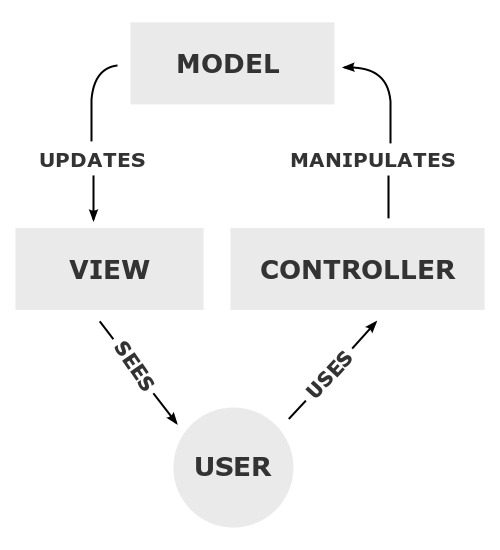
\includegraphics[keepaspectratio, width=0.5\textwidth]{mvc}
	\src{https://en.wikipedia.org/wiki/Model-view-controller}{10.12.2017}
	\caption{Interaktion innerhalb des Model-View-Controller Prinzips}
	\label{fig:mvc}
\end{figure}

Dieses Kapitel entspricht der dritten Phase des \hcdp{} und verfolgt das Ziel, einen ersten benutzbaren Prototyp zu schaffen, der die in \autoref{chap:problem} beschriebenen Probleme möglichst gut löst. 
Anschließend soll die \emph{Android-Library}, welche bei der Entwicklung des Prototyps entsteht, in die vorhandene App integriert werden.
Auf diese Weise kann der Prototyp bereits im Arbeitsalltag der Monteure getestet werden.
Dies ermöglicht das Identifizieren von eventuell neuen Usability-Problemen, die während der initialen Beobachtung noch nicht aufgefallen sind. \\

Alle Erkenntnisse aus dieser ersten \emph{Testing}-Phase werden anschließend mit in \emph{Observation} der zweiten Iteration des \hcdp{} Zyklus übernommen, um diese in einem verbesserten Prototyp zu lösen.
Das Ziel dieses Kapitels ist, einen funktionierenden Prototyp in Form einer Android-Library zu entwickeln, welcher sich in die bestehende Android-Applikation integrieren lässt und die Bewertungskriterien aus \autoref{chap:eval} erfüllt.

\section{Implementation}\label{sec:pro1}
In \autoref{chap:concept} wurden Umsetzungsmöglichkeiten für die verschiedenen Bewertungskriterien aus \autoref{sec:criteria} ausgearbeitet.
Diese sollen in die Implementierung des ersten Prototyps einfließen und so einen Grundstein für eine positive Benutzererfahrung der App legen. \\

Der erste Prototyp wurde am 16. Dezember 2017 fertiggestellt und in die bestehende Android-App eingebunden. \\

\noindent
Zusätzlich wurde der Aufbau des Projekts in der \emph{Unified Modelling Language}, kurz \emph{UML}, modelliert.
Dies ermöglicht bereits vor der eigentlichen Implementierung wichtige Begriffe und mögliche Beziehungen festzulegen, und einen Überblick über die benötigten Klassen zu bekommen.

\begin{figure}[h]
  \centering
  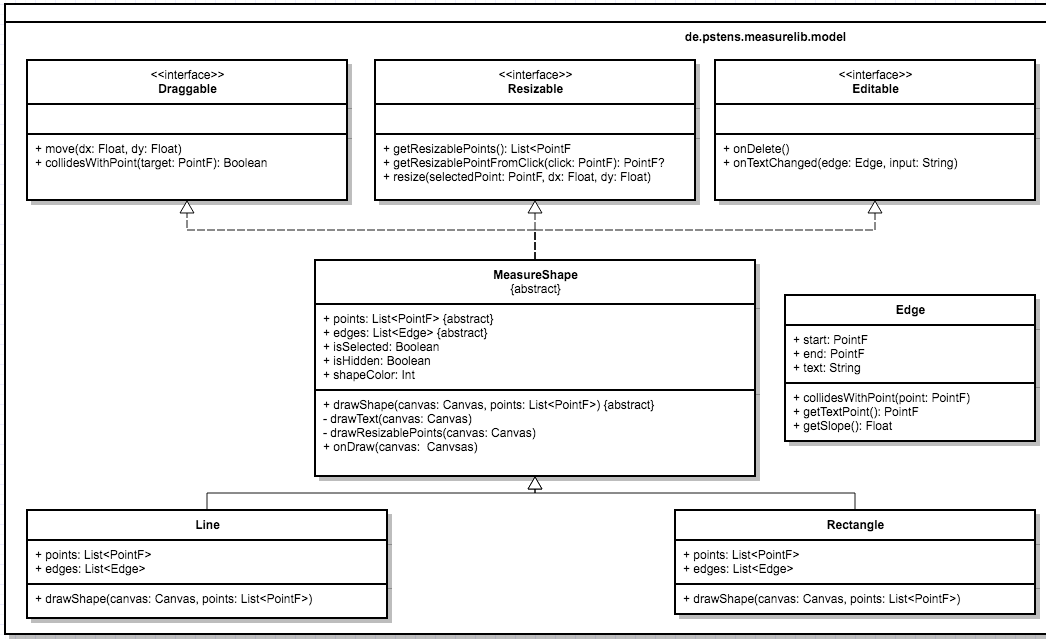
\includegraphics[keepaspectratio, width=\textwidth]{prototype1/shape}
  \caption{Ausschnitt aus der Datenmodell-Komponente des UML-Diagramms}
  \label{fig:shape}
\end{figure}

\noindent
Die Komponente des \emph{Datenmodells} sah dabei wie folgt aus (eine vollständige Version des UML-Diagramms befindet sich in \autoref{chap:uml}):
In \autoref{fig:shape} ist die abstrakte Klasse \emph{MeasureShape} zu erkennen, welche die Oberklasse der beiden Formen \emph{Line} und \emph{Rectangle} darstellt.
\emph{MeasureShape} vererbt die abstrakten Attribute \emph{points} und \emph{edges} an ihre Unterklassen, die diese Attribute überschreiben müssen.
Außerdem muss die öffentliche Methode \emph{drawShape(...)} von beiden Unterklassen implementiert werden.
Dies sorgt dafür, dass jede Unterklasse selber dafür ``verantwortlich'' ist, wie und wohin ihre Form gezeichnet wird.
\emph{MeasureShape} implementiert die drei \emph{Interfaces} \emph{Draggable, Resizable} und \emph{Editable}, welche Schnittstellen zum Verschieben, Vergrößern und Editieren von Formen bereit stellen. \\

\noindent
Eine weitere Klasse im \emph{Datenmodell} ist \emph{UserAction} (siehe \autoref{fig:model}).
Diese ist eine versiegelte (\emph{sealed}) Oberklasse, welche die verschiedenen Benutzeraktionen darstellt.
Versiegelt bedeutet in diesem Kontext, dass nur Klassen, welche im \emph{Scope} der Oberklasse liegen, von dieser erben können.
Folgende sechs Benutzeraktionen können in der Implementierung des ersten Prototyps über die Undo/Redo-Funktion rückgängig gemacht oder wiederhergestellt werden:

\begin{itemize}
  \item Verschieben von Formen (\emph{DraggedShape})
  \item Hinzufügen von Formen (\emph{AddedShape})
  \item Löschen von Formen (\emph{RemovedShape})
  \item Vergrößern bzw. verkleinern von Formen (\emph{ResizedPoint})
  \item Ändern des Textes (\emph{ChangedText})
  \item Ändern der Farbe (\emph{ChangedColor})
\end{itemize}

\noindent
Funktional beschränkt sich die Implementierung des ersten Prototyps zunächst auf das Zeichnen von einfachen Linien und Vierecken, sowie das anschließende Beschriften um Messwerte einzutragen.
Zum schnellen und präzisen Zeichnen der Formen wird eine Zoom-Linse (siehe \autoref{fig:draw1}), wie sie in allen drei Apps aus \autoref{chap:eval} umgesetzt wurde, verwendet.
Der Prototyp verfügt über zwei verschiedene Modi, den Zeichen- und Text-Modus, zwischen denen mit Hilfe des \emph{Floating Action Buttons} im unteren rechten Bildschirmbereich umgeschaltet werden kann (siehe \autoref{fig:all1}).
Zudem kann der Benutzer über einen weiteren \emph{Floating Action Button} im unteren linken Bildschirmbereich jederzeit ein neues Bild aufnehmen, oder ein bereits vorhandenen in die App importieren.

\begin{figure}[h]
  \begin{subfigure}[t]{0.4\textwidth}
    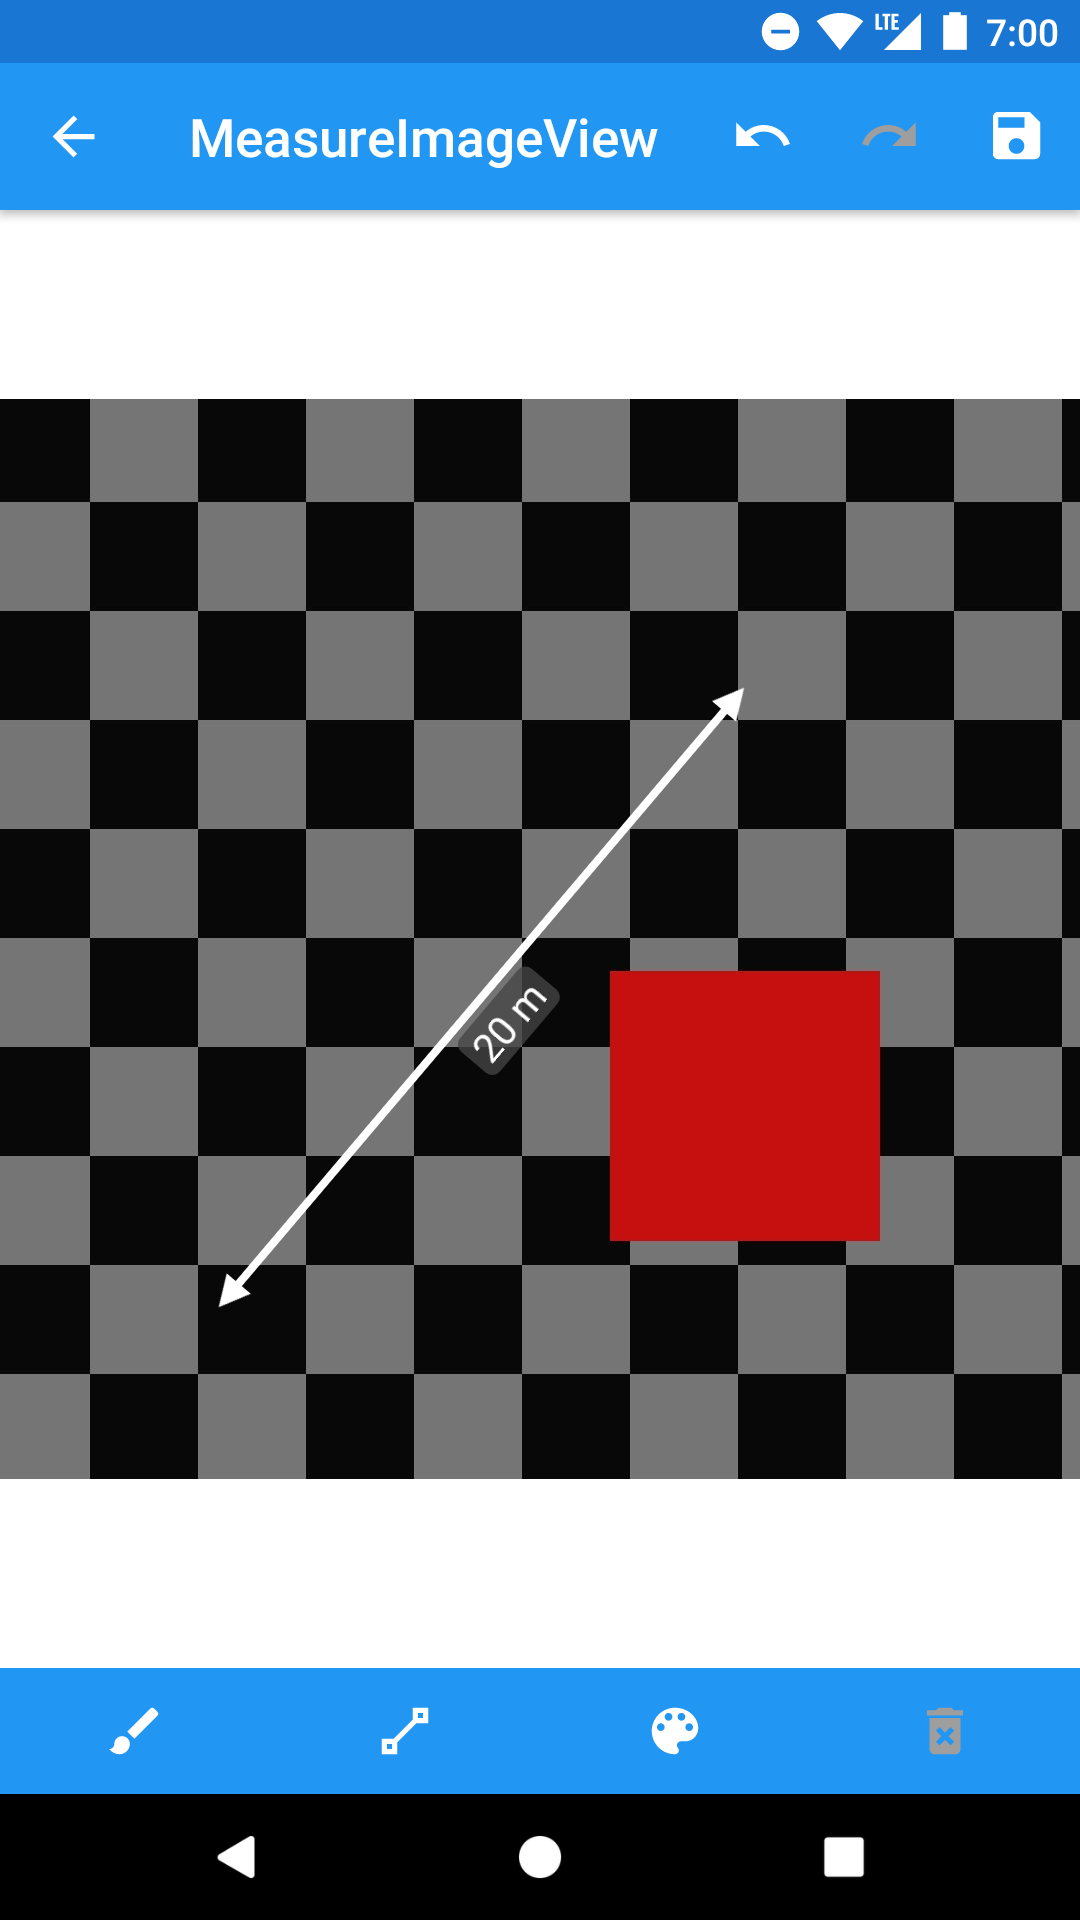
\includegraphics[keepaspectratio, width=\textwidth]{prototype1/all}
    \caption{Erster Prototyp mit bereits eingezeichneter Linie}
    \label{fig:all1}
  \end{subfigure}
  \begin{subfigure}[t]{0.4\textwidth}
    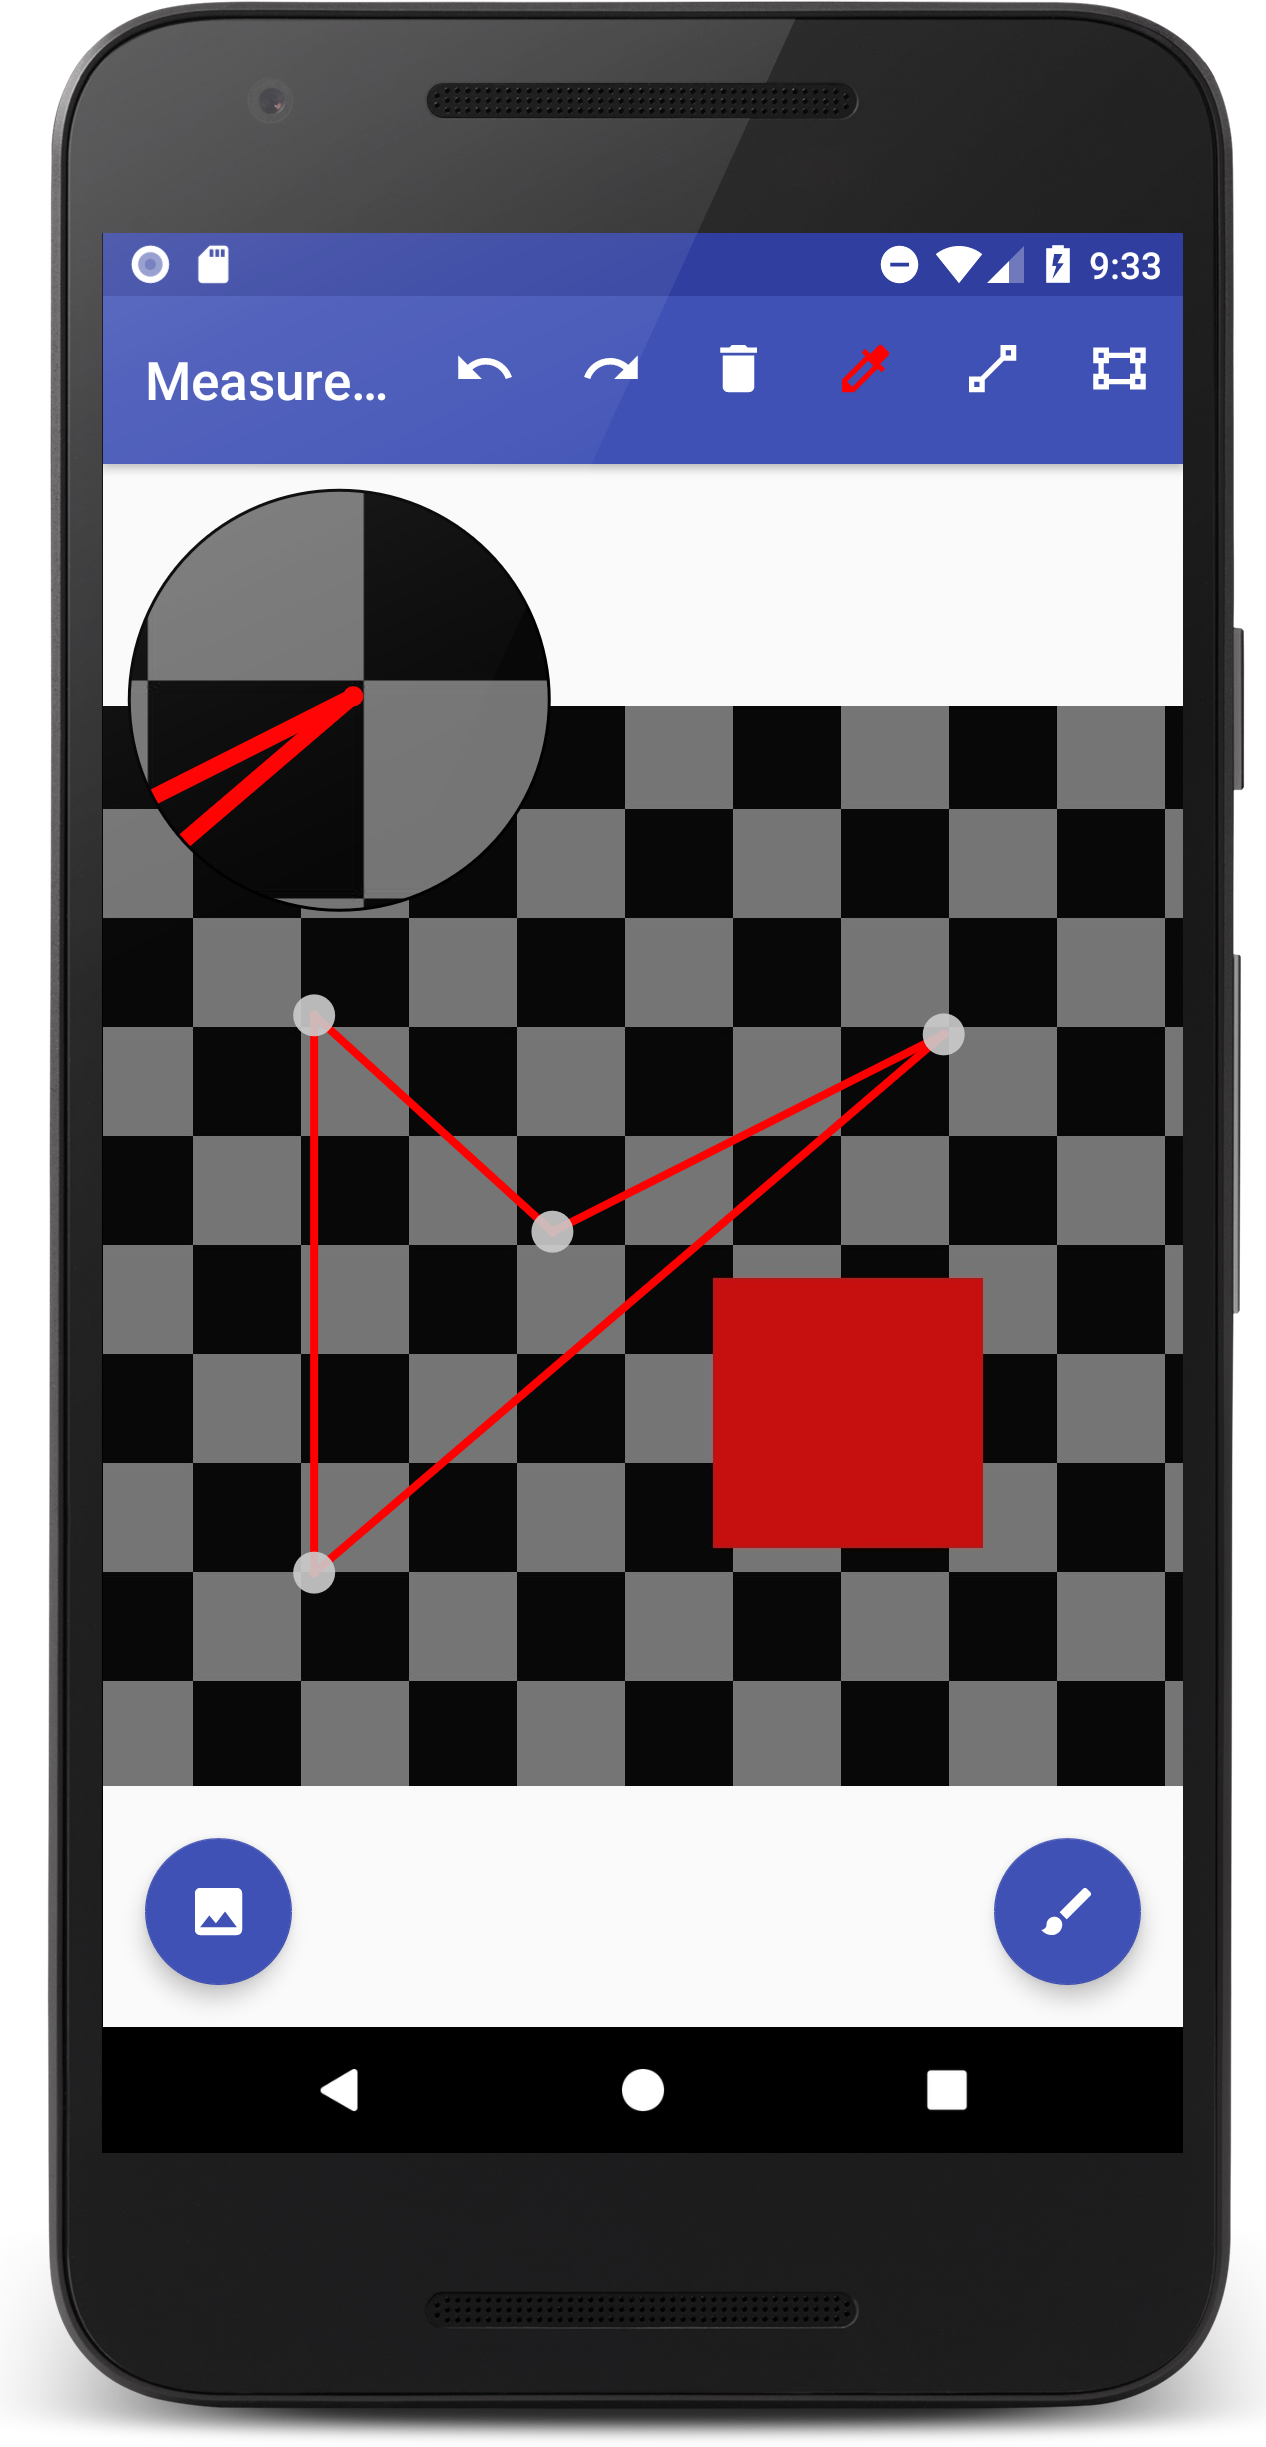
\includegraphics[keepaspectratio, width=\textwidth]{prototype1/rect}
    \caption{Zoom-Linse beim Zeichnen eines Vierecks}
    \label{fig:draw1}
  \end{subfigure}
  \centering
  \caption{Erster Prototyp bei eingezeichneter Linie und beim Zeichnen eines Vierecks}
\end{figure}

Undo- sowie Redo-Funktion befinden auf dedizierten \emph{Buttons} in der Menüleiste der App (siehe \autoref{fig:all1}).
Hier gibt es außerdem jeweils einen Button, um ausgewählte Formen zu löschen, die Zeichenfarbe zu ändern, oder eine andere Form zum Zeichnen auszuwählen. \\

\begin{wrapfigure}{R}{0.4\textwidth}
  \centering
  \includegraphics[keepaspectratio, width=0.4\textwidth]{prototype1/color}
  \caption{Geöffneter Farbauswahl-Dialog}
  \label{fig:color1}
\end{wrapfigure}

Beim Auswählen des Farb-Icons in der Menüleiste öffnet sich ein modaler Dialog, der es dem Benutzer ermöglicht, die gewünschte Farbe auszuwählen (siehe \autoref{fig:color1}).
Diese Farbe wird als Standardfarbe für alle neuen Formen genutzt.
Falls vor dem Öffnen des Dialogs eine Form markiert wurde, wird diese ebenfalls mit der ausgewählten Farbe eingefärbt. \\

Graue Indikatoren an den Eckpunkten der aktuell ausgewählte Form sollen dem Nutzer verdeutlichen, dass diese mit Hilfe der Indikatoren in ihrer Größe und Position bearbeitet werden kann. (siehe \autoref{fig:draw1}).
Um Formen zu beschriften bietet sich dem Benutzer im Text-Modus die Möglichkeit, Kanten mittels eines Eingabe-Dialogs zu annotieren.
Hierzu öffnet sich durch einen langen Klick auf die Kante einer Form im Text-Modus ein modaler Dialog, welcher die Messwerte des Nutzers entgegennimmt.
Eingetragene Messwerte werden anschließend neben der zuvor ausgewählten Kante im Bild dargestellt. 

% \begin{figure}[h]
% \begin{subfigure}[t]{0.4\textwidth}
% 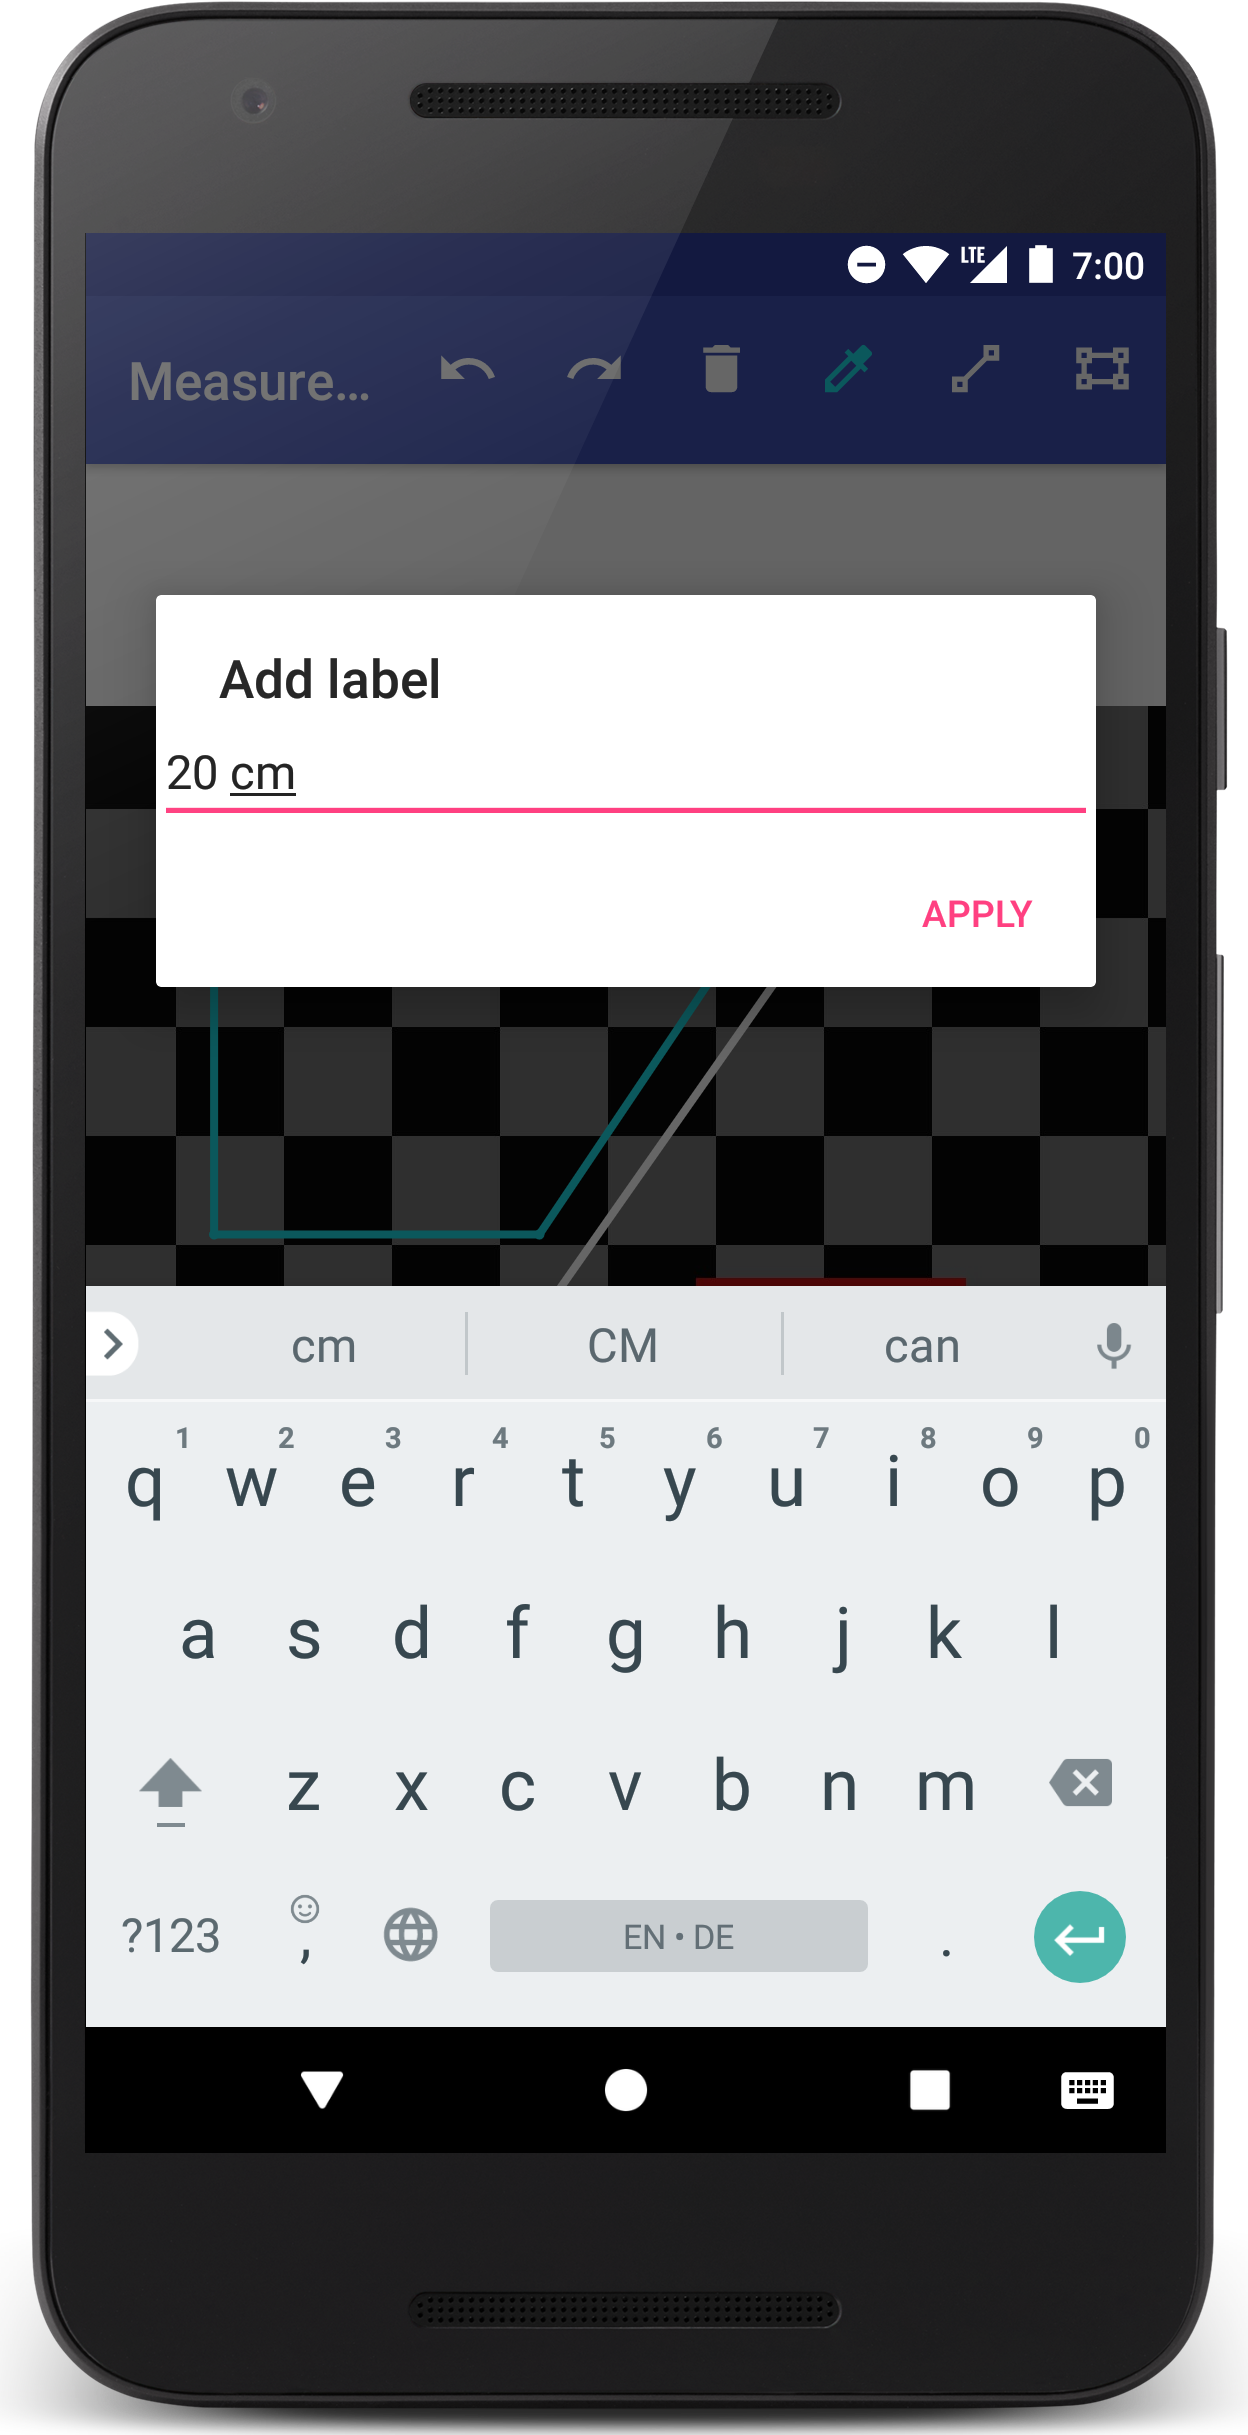
\includegraphics[keepaspectratio, width=\textwidth]{prototype1/labeling}
% \caption{Dialog zum Eintragen von Messwerten}
% \label{fig:labeling1}
% \end{subfigure}
% \begin{subfigure}[t]{0.4\textwidth}
% 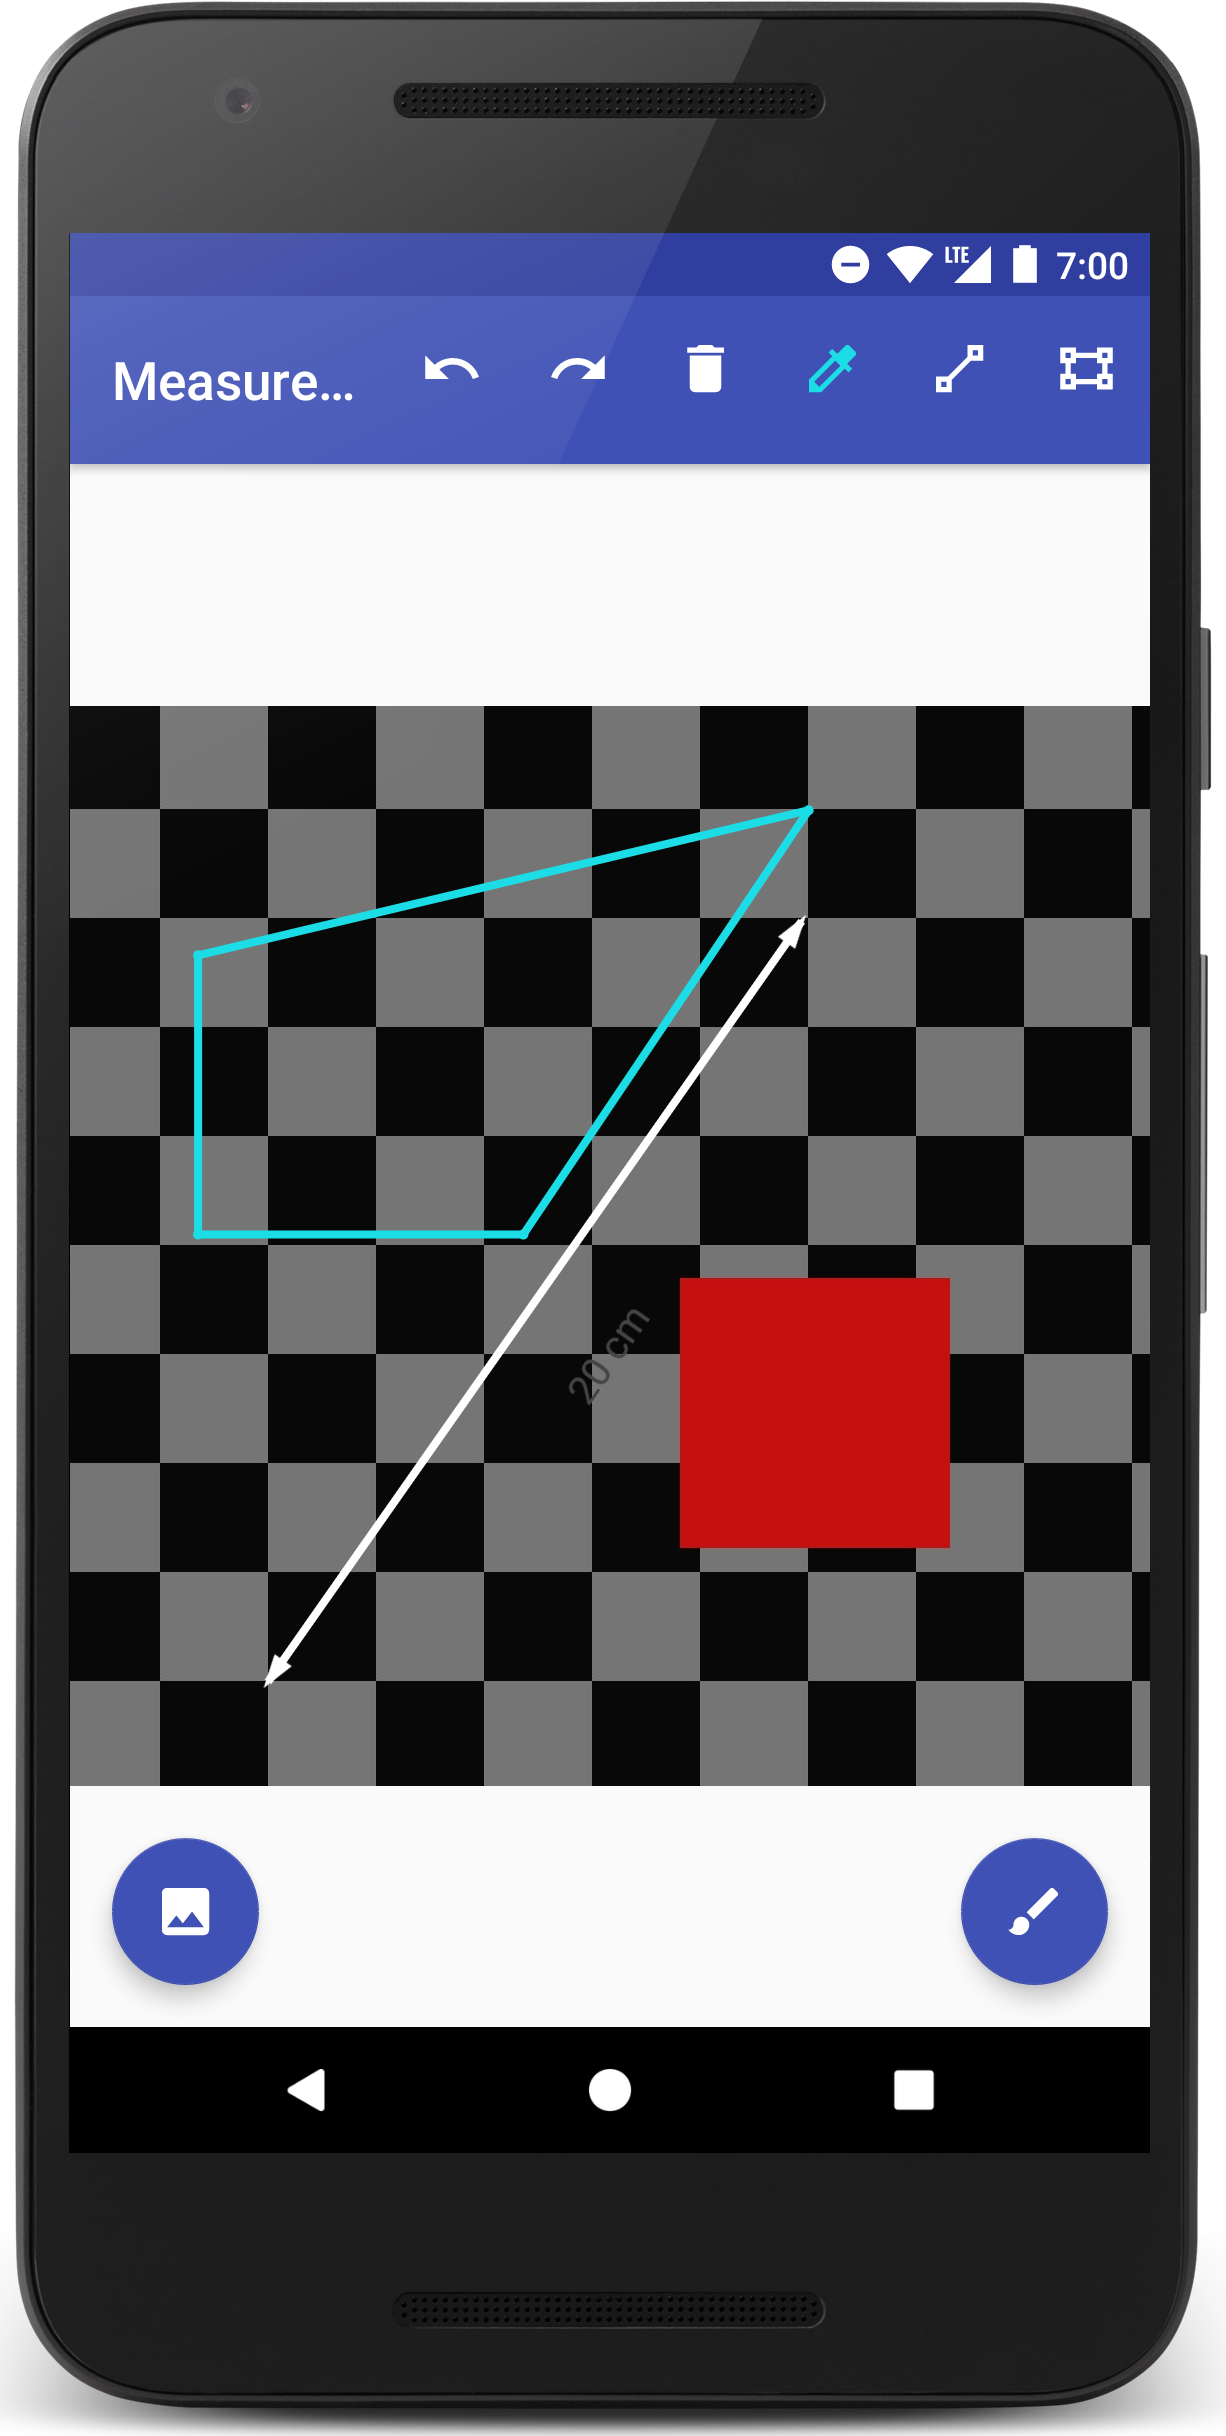
\includegraphics[keepaspectratio, width=\textwidth]{prototype1/label}
% \caption{Linie mit eingetragenem Messwert}
% \label{fig:label1}
% \end{subfigure}
% \centering
% \caption{Eintragen und Anzeigen von Messwerten im ersten Prototyp}
% \end{figure}

\section{Test}\label{sec:test1}
Zum Testen des Prototyps wurde dieser in die App der beiden Geschäftsführer der \emph{Fa.} \vr{} (siehe \autoref{table:testers}) eingebunden.
Testperson 1, André Vermeulen, repräsentiert hierbei den ``Poweruser'' der App, wohingegen Testperson 2, Sebastian Wiesbrock, die App gelegentlich nutzt.
Beiden Testern wurde zur Nutzung des Prototyps weder eine verbale noch schriftliche Hilfestellung zur Verfügung gestellt. \\

\begin{table}[h]
  \centering
  \begin{tabular}{l | c | c}
    \hline
    \textbf{Testperson} & \textbf{1} & \textbf{2} \\
    \hline
    \textbf{Name} & André Vermeulen & Sebastian Wiesbrock \\
    \hline
    \textbf{Rolle} & Geschäftsleitung & Geschäftsleitung \\
    \hline
    \textbf{Alter} & 45 &  ?? \\
    \hline
    \textbf{Nutzungsgrad der App} & hoch & mittel \\
    \hline
  \end{tabular}
  \caption{Demografische Daten der Testpersonen}
  \label{table:testers}
\end{table}

Nachdem die beiden Tester den Prototyp zwei Tage in ihren Arbeitsalltag integriert haben, wurden am 18. Dezember die Testergebnisse gesammelt:

Nach Aussage beider Testpersonen, haben die \emph{Floating Action Buttons} sich bei der Benutzung der App als großes Hindernis herausgestellt.
So sei nicht intuitiv klar, dass die App über zwei verschiedene Modi, nämlich den Zeichen- und Text-Modus, verfügt.
Zudem sei unklar, dass man über einen Klick auf den rechten \emph{Floating Action Button} zwischen den beiden Modi wechseln kann. \\

Ein weiteres Problem ergab sich laut Testperson 1 bei der Benutzung der App auf seinem Tablet.
So seien sämtliche Texte nur schwer lesbar, und die Punkte zum Verändern der Formen so klein, dass sie nur mühsam und mit viel Konzentration mit dem Finger zu treffen seien. \\

Darüber hinaus schilderten beide Testpersonen, dass eingetragene Messwerte auf Bildern, die in dunkleren Lichtverhältnissen aufgenommen wurden, nur schlecht lesbar seien.
Hier setze sich die Textfarbe zu schlecht vom Hintergrund ab. \\

Zusätzlich zu den identifizierten Usability-Problemen kam bei beiden Testern der Wunsch nach neuen Funktionen auf, die sie sich als nützliche Erweiterungen hinsichtlich ihres Arbeitsalltags vorstellen konnten.
So wünschten sich beide Testpersonen einerseits die Möglichkeit, Formen mit bereits vorhandenen Gerüsttypen zu verbinden und in den Meta-Daten des Bildes zu speichern.
Andererseits wurde angemerkt, dass es sinnvoll sei, Bilder vor dem Bearbeiten über eine weitere Oberfläche zunächst in die gewünschte Größe und Form schneiden zu können, da es oftmals auf der Baustelle vorkomme, dass die aufgenommenen Bilder nicht nur das gewünschte Gerüst, sondern auch andere Objekte, die für das Bild nicht relevant sind, beinhalten. \\

Die Ursachen und mögliche Lösungsideen der Probleme, die während dieser Testphase identifiziert wurden, sollen im nächsten Abschnitt in einer weiteren Iteration des \hcdp{} ausgewertet und mit Hilfe eines zweiten Prototyps gelöst werden.

\chapter{Zweite Iteration - Intuitive Bedienbarkeit}\label{chap:pro2}
In \autoref{sec:test1} haben sich während der Testphase des ersten Prototyps sowohl neue Probleme als auch fehlende Funktionen identifizieren lassen.
Diese sollen bei der Entwicklung eines zweiten Prototyps in diesem Abschnitt berücksichtigt werden. 
Hierzu werden die vier Phasen des \hcdp{} ein weiteres Mal durchlaufen.

\section{Observation}
Um einen Überblick über die Test-Ergebnisse aus \autoref{sec:test1} herzustellen, werden diese im Nachfolgenden zunächst aufgelistet und anschließend weiter evaluiert:

\begin{itemize}
  \item Bedienung der App über \emph{FAB} nicht intuitiv
  \item Text- und Formelemente auf Tablet-Geräten nicht gut bedienbar
  \item Eingetragene Messwerte bei dunklem Hintergrund nicht gut erkennbar
  \item Anwenderwunsch: Zuordnen von Gerüsttypen zu Formen
  \item Anwenderwunsch: Zuschneiden und Rotieren des Bildes
\end{itemize}

\noindent
Zunächst auffällig ist, dass beide Testpersonen in \autoref{sec:test1} die \emph{Floating Action Buttons} als Hindernis bei der Bedienung der App beschreiben.
Da alle möglichen Aktionen erst dann sichtbar werden, wenn der \emph{FAB} angeklickt wird und sonst nur ein einzelnes Icon angezeigt wird, wird dem Nutzer keine angemessene Rückmeldung über den aktuellen Systemzustand gegeben.
Außerdem wird hierdurch keine ausreichende Hilfestellung zu den vorhandenen Funktionen und wie diese zu benutzen sind gegeben.
(Nielsen~\autoref{itm:N1} \& \autoref{itm:N10}) \\

Ein weiterer Punkt, der in \autoref{sec:test1} während der \emph{Testing}-Phase negativ aufgefallen ist, ist die Benutzung der App auf Tablet-Geräten.
Damit Endgeräte mit einer großen Bildschirmdiagonale trotzdem über eine scharfe Auflösung verfügen, besitzen diese mehr Pixel pro Zentimeter bzw. eine höhere Pixeldichte.
Da die UI-Elemente im ersten Prototyp mit Hilfe von \emph{Pixeln}, welche von Android zur Laufzeit nicht für die entsprechenden Bildschirmgrößen optimiert werden, modelliert worden sind, werden UI-Elemente auf Tablet-Geräten kleiner dargestellt, als auf normalen Smartphones.
Dies erschwert die Benutzung der App auf Tablets, da Texte nur mühsam zu lesen und Formen schwierig auszuwählen sind.
So werden hier einerseits potentielle Fehlerquellen generiert, andererseits wird das Nutzungserlebnis auf Tablet-Geräten negativ beeinflusst.
(Nielsen~\autoref{itm:N5} \& \autoref{itm:N13}) \\

Darüber hinaus zeigen die Testergebnisse, dass die Testpersonen Probleme beim Erkennen von eingetragenen Messwerten auf dunklen Bildern haben.
Die schlechte Lesbarkeit der Messwerte resultiert wahrscheinlich aus der grauen Textfarbe, welche unabhängig vom Farbraum des Bildes festgelegt ist.
Zudem fehlt ein Hintergrund, der unter dem Text liegt und diesen so vom eigentlichen Bild abhebt.
(Nielsen~\autoref{itm:N12}). \\

Zusätzlich zu den Problemen, die während der Testphase des ersten Prototyps identifiziert worden sind, haben sich bei den Testpersonen Wünsche für Funktionen, die nicht in der Implementierung des ersten Prototyps zu finden sind, aber im Alltag regelmäßig benötigt werden, herauskristallisiert. 
So soll der Prototyp zum Einen um eine Funktionen erweitert werden, die es ermöglicht, eingetragene Formen mit vordefinierten Gerüsttypen zu verknüpfen.
Zum Anderen soll die Möglichkeit bestehen, Bilder beim Import in die App in die gewünschte Größe und Form schneiden zu können.

\section{Idea Generation}\label{sec:idea2}
Um dem Benutzer jederzeit eine klare und einfache Rückmeldung über den aktuellen Systemzustand und die darin ausführbaren Aktionen zu geben, bietet es sich an, eine Statusleiste am unteren Bildschirmrand zu verankern.
Diese soll mit Hilfe von unterscheidbaren, aber intuitiv verständlichen Icons, über den aktuellen Modus informieren und zugleich nicht-benutzbare Aktionen nicht-auswählbar gestalten.
Die \mg{} suggerieren hierfür die Nutzung einer sogenannten \emph{Bottom navigation}\urlnote{https://material.io/guidelines/components/bottom-navigation.html}{02.01.2018}.
Diese kann, so die \mg{}, dazu eingesetzt werden, um die Erkundung von Apps einfach zu gestalten und den Wechsel zwischen den Ansichten auf der obersten Ebene einer App zu beschleunigen \citep{BN18}. \\

Für eine bessere und einfachere Benutzung der App auf Tablet-Geräten kann eine zweite Benutzeroberfläche, die nur auf Tablet-Geräten angezeigt wird, in die App eingebunden werden. 
Hierzu heißt es in  den ``Developer Guides'' von Android zur Unterstützung von verschiedenen Bildschirmgrößen\urlnote{https://developer.android.com/guide/practices/screens_support.html}{02.01.2018} im Abschnitt ``Supporting Multiple Screens'', dass Entwickler verschiedene Konfigurationskriterien festlegen können, die zur Laufzeit der App ausgewertet werden, und in der Benutzung verschiedener Ressourcen wie zum Beispiel der angezeigten Oberfläche resultieren \citep[How to Support Multiple Screens]{SS18}.
So gibt beispielsweise das Kriterium \emph{sw720dp} an, dass alle Geräte, die eine Bildschirmbreite von mindestens $720dp$ besitzen, die Ressourcen benutzen, welche mit \emph{sw720dp} gekennzeichnet sind.
Dies kann dazu genutzt werden, um eine dedizierte Benutzeroberfläche mit größeren Icons und Texten für Tablet-Geräte bereit zu stellen.
Alternativ besteht die Möglichkeit, eine Oberfläche für alle Geräte zu nutzen, aber die Größe diverser Text- und Formelemente mit der Bildschirmgröße zu skalieren.
Die ``Developer Guidelines'' schlagen hierzu die Nutzung sogenannter ``dichteunabhängiger Pixel'' vor \citep[Density Independence]{SS18}.
Diese können dazu genutzt werden, um dem System die Skalierung sämtlicher UI-Elemente zu überlassen, was zur Folge hat, dass diese auf unterschiedlichen Bildschirmgrößen gleich groß dargestellt werden.
\\

Die schlechte Erkennbarkeit von eingetragenen Messwerten auf Bildern mit dunklem Hintergrund sollen durch das Anpassen der Textfarbe in Kombination mit der Benutzung eines Texthintergrundes gelöst werden.
\citeauthor{Jankowski10} schreiben hierzu in ihrer Arbeit ``Integrating Text with Video and 3D Graphics: The Effects of Text Drawing Styles on Text Readability'' aus dem Jahr 2010, dass ein Plakatwand-ähnlicher Zeichenstil zur schnellsten und genausten Erkennbarkeit des Textes führt \citep[Seite 1330]{Jankowski10}.
Zudem führe die Benutzung von weißem Text auf einem halbtransparenten schwarzen Hintergrund zu einer deutlich schnelleren und genaueren Erkennbarkeit des Textes als die Verwendung von schwarzer Schrift auf weißem Hintergrund \citep[Seite 1328]{Jankowski10}. \\

Um Formen direkt den passenden Gerüsttypen zuzuordnen, bietet sich die Verwendung eines modalen Dialogs an.
Dieser könnte zum Beispiel bei einem langen Klick auf die gewünschte Form angezeigt werden, und in einem \emph{Dropdown} vorhandene Gerüsttypen zur Auswahl anbieten.
Falls ein langer Klick auf die Form bei der ersten Benutzung zu un-intuitiv ist, würde sich ein \emph{Button} anbieten, der nur dann auswählbar ist, wenn zuvor eine Form markiert wurde.
Zudem sollte an der Form erkenntlich werden, dass sie bereits mit einem Gerüsttyp verknüpft ist. \\

Das Schneiden und Rotieren von Bildern kann einerseits durch die Benutzung der im Android-System vorhandenen \emph{Crop-Activity} realisiert werden, andererseits würde sich auch die Benutzung einer \emph{Open-Source Android-Library} für das Schneiden von Bildern anbieten.
Die Verfügbarkeit der von Android bereitgestellten \emph{Crop-Activity} ist jedoch vom Gerätehersteller und der verwendeten Android-Version abhängig.
Hierdurch kann nicht sichergestellt werden, dass die Funktion auf allen Geräten funktioniert.
In einem Blog-Eintrag der Seite ``The CommonsBlog'' mit dem Titel ``No, Android Does *Not* Have a Crop Intent'' steht hierzu folgendes \citep{Commonsware13}:
\begin{quote}
  ``Many developers are calling startActivity() on an Intent with an action of com.android.camera.action.CROP.
  [...] Devices lacking this app will not respond to this undocumented Intent action, and your app will crash.'' 
\end{quote}

\noindent
Deshalb bietet sich die Verwendung einer \emph{Open-Source Android-Library} an.

\section{Prototyping}
Der zweite Prototyp wurde am 3. Januar 2018 fertiggestellt, und umfasst die Implementierung der in \autoref{sec:idea2} gesammelten Ideen. \\

\begin{figure}[h]
  \begin{subfigure}[t]{0.4\textwidth}
    \centering
    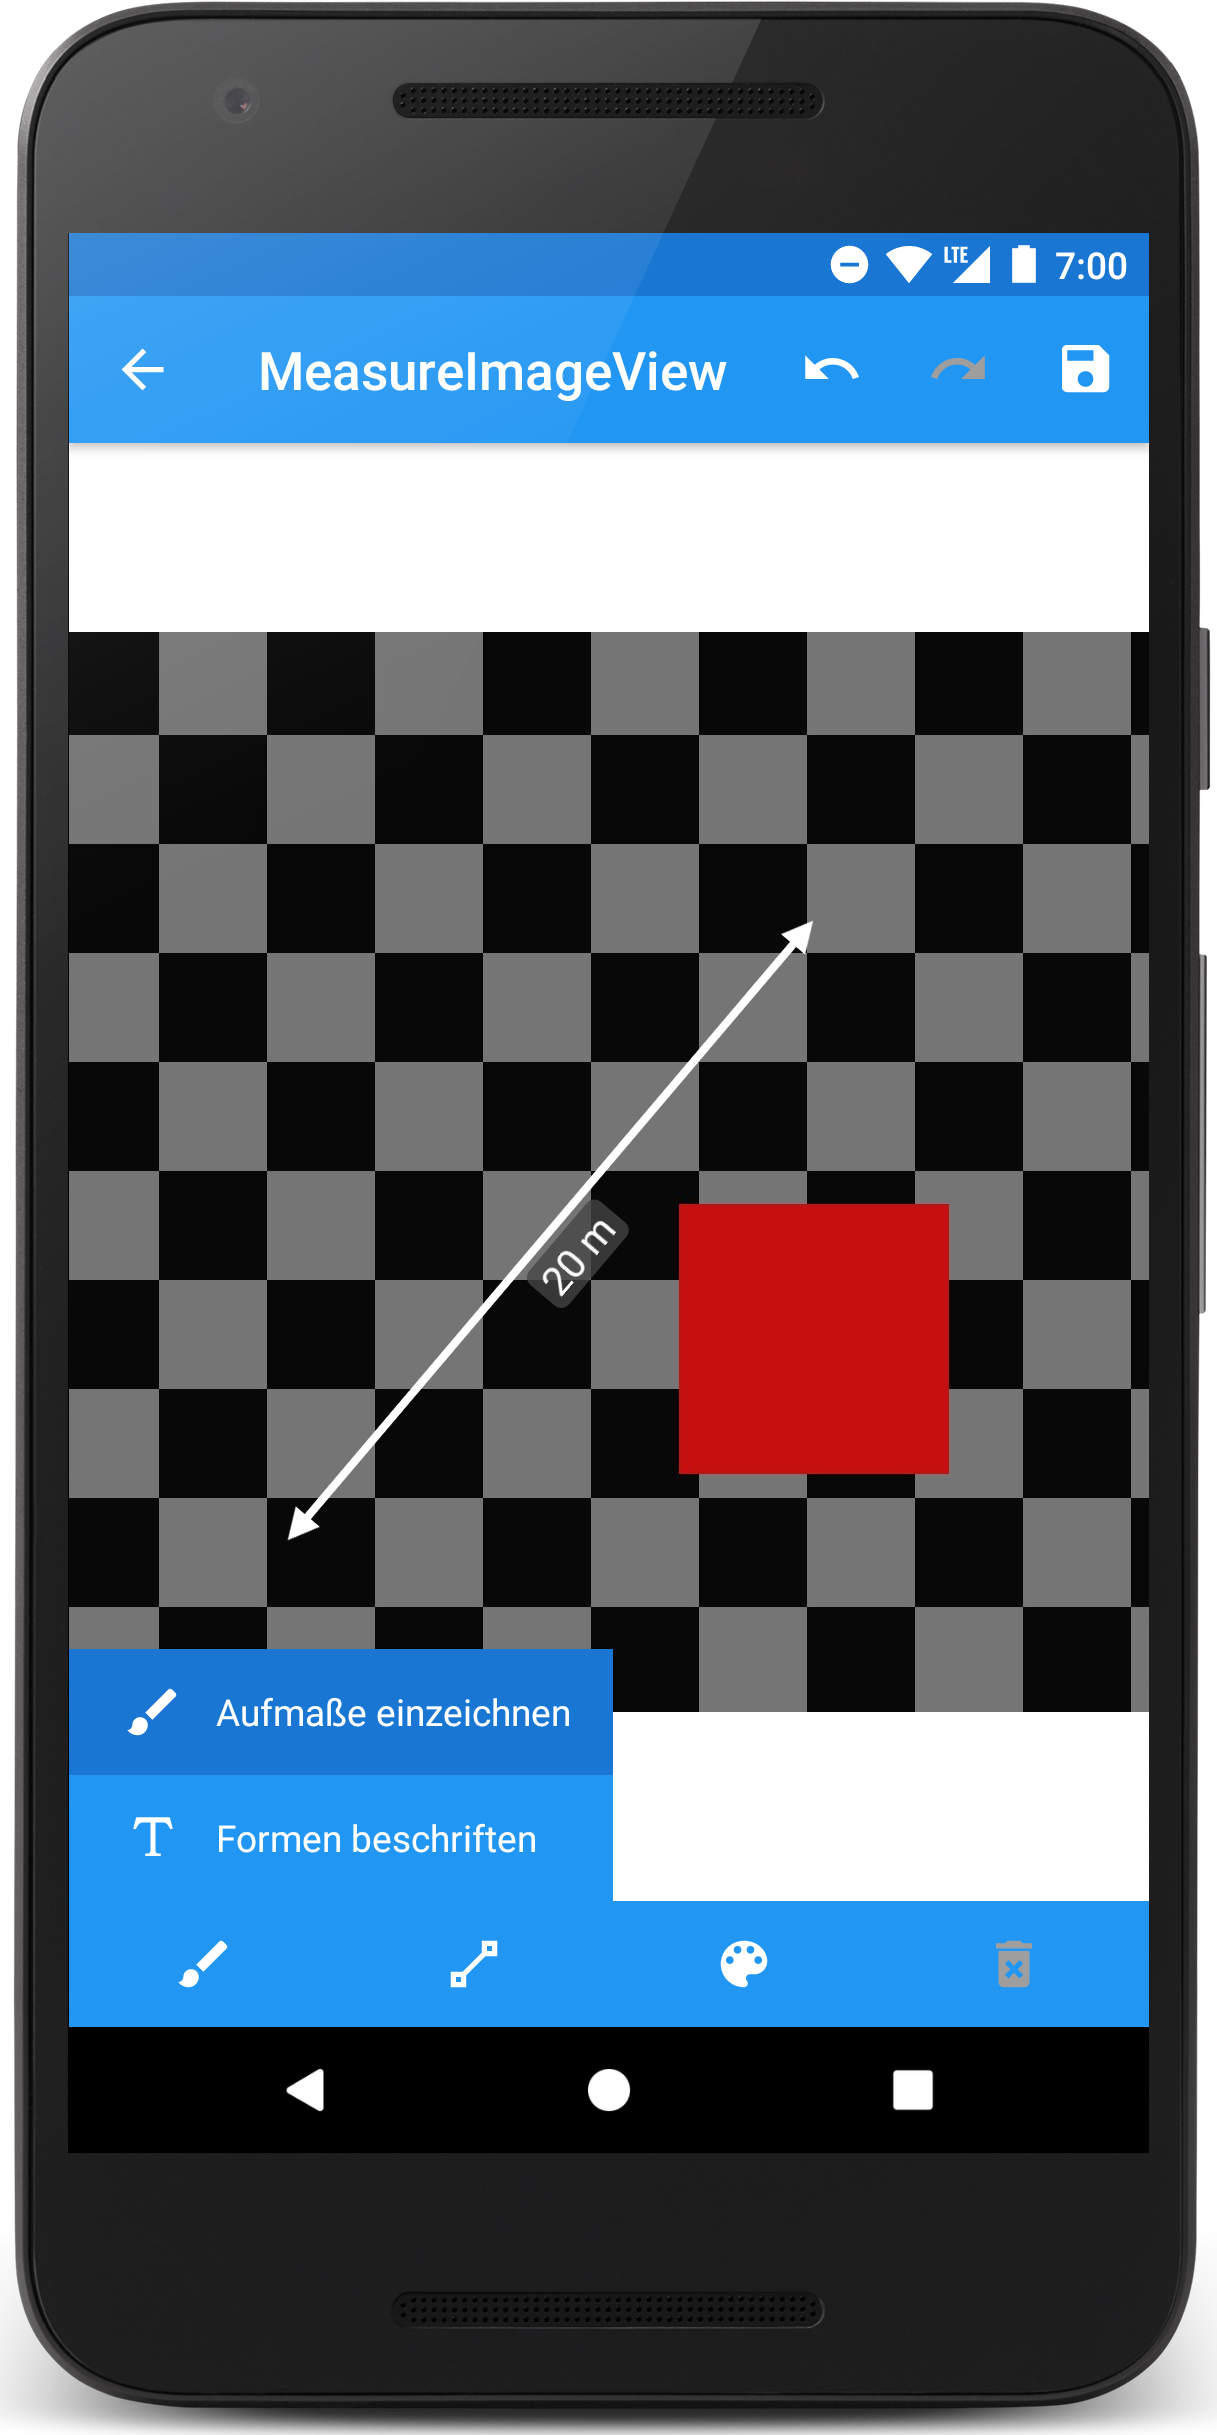
\includegraphics[keepaspectratio, width=\textwidth]{prototype2/expanded_mode}
    \caption{Statusleiste im Zeichen-Modus mit Popup-Dialog zur Auswahl des Modus}
    \label{fig:mode2}
  \end{subfigure}
  ~
  \begin{subfigure}[t]{0.4\textwidth}
    \centering
    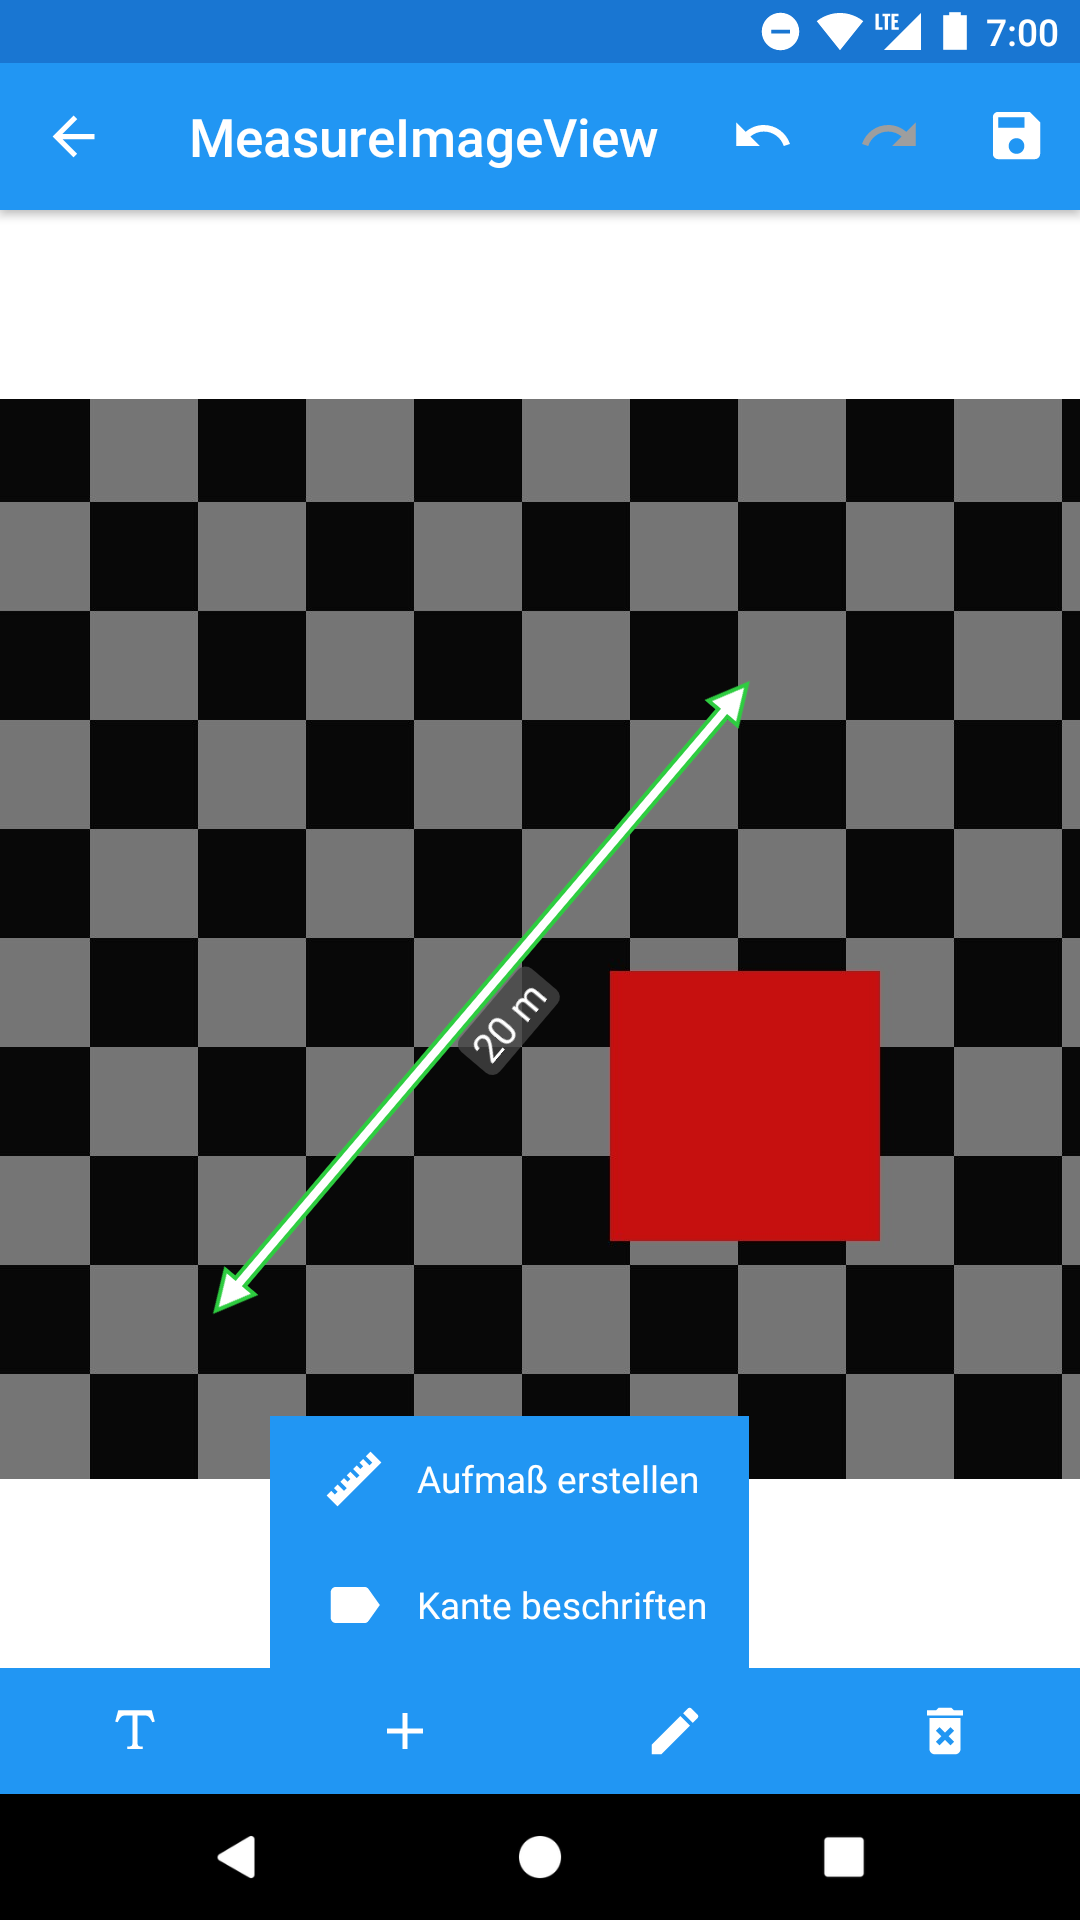
\includegraphics[keepaspectratio, width=\textwidth]{prototype2/label_popup}
    \caption{Statusleiste im Text-Modus mit Popup-Dialog zur Beschriftung der ausgewählten Form}
    \label{fig:labelp2}
  \end{subfigure}
  \centering
  \caption{Bedienung der Statusleiste im zweiten Prototyp}
  \label{fig:bar2}
\end{figure}

Die Statusleiste wurde durch eine \emph{Bottom-Navigation Bar} am unteren Bildschirmrand umgesetzt (siehe \autoref{fig:bar2}).
Diese besteht aus vier verschiedenen Icons, die nur dann auswählbar sind, wenn die entsprechende Aktion im aktuellen Systemzustand durchführbar ist.
Das Pinsel- bzw. Text-Icon ganz links in der Leiste ermöglicht das Wechseln zwischen dem Zeichen- und Text-Modus (siehe \autoref{fig:mode2}). \\

\begin{wrapfigure}{R}{0.4\textwidth}
  \centering
  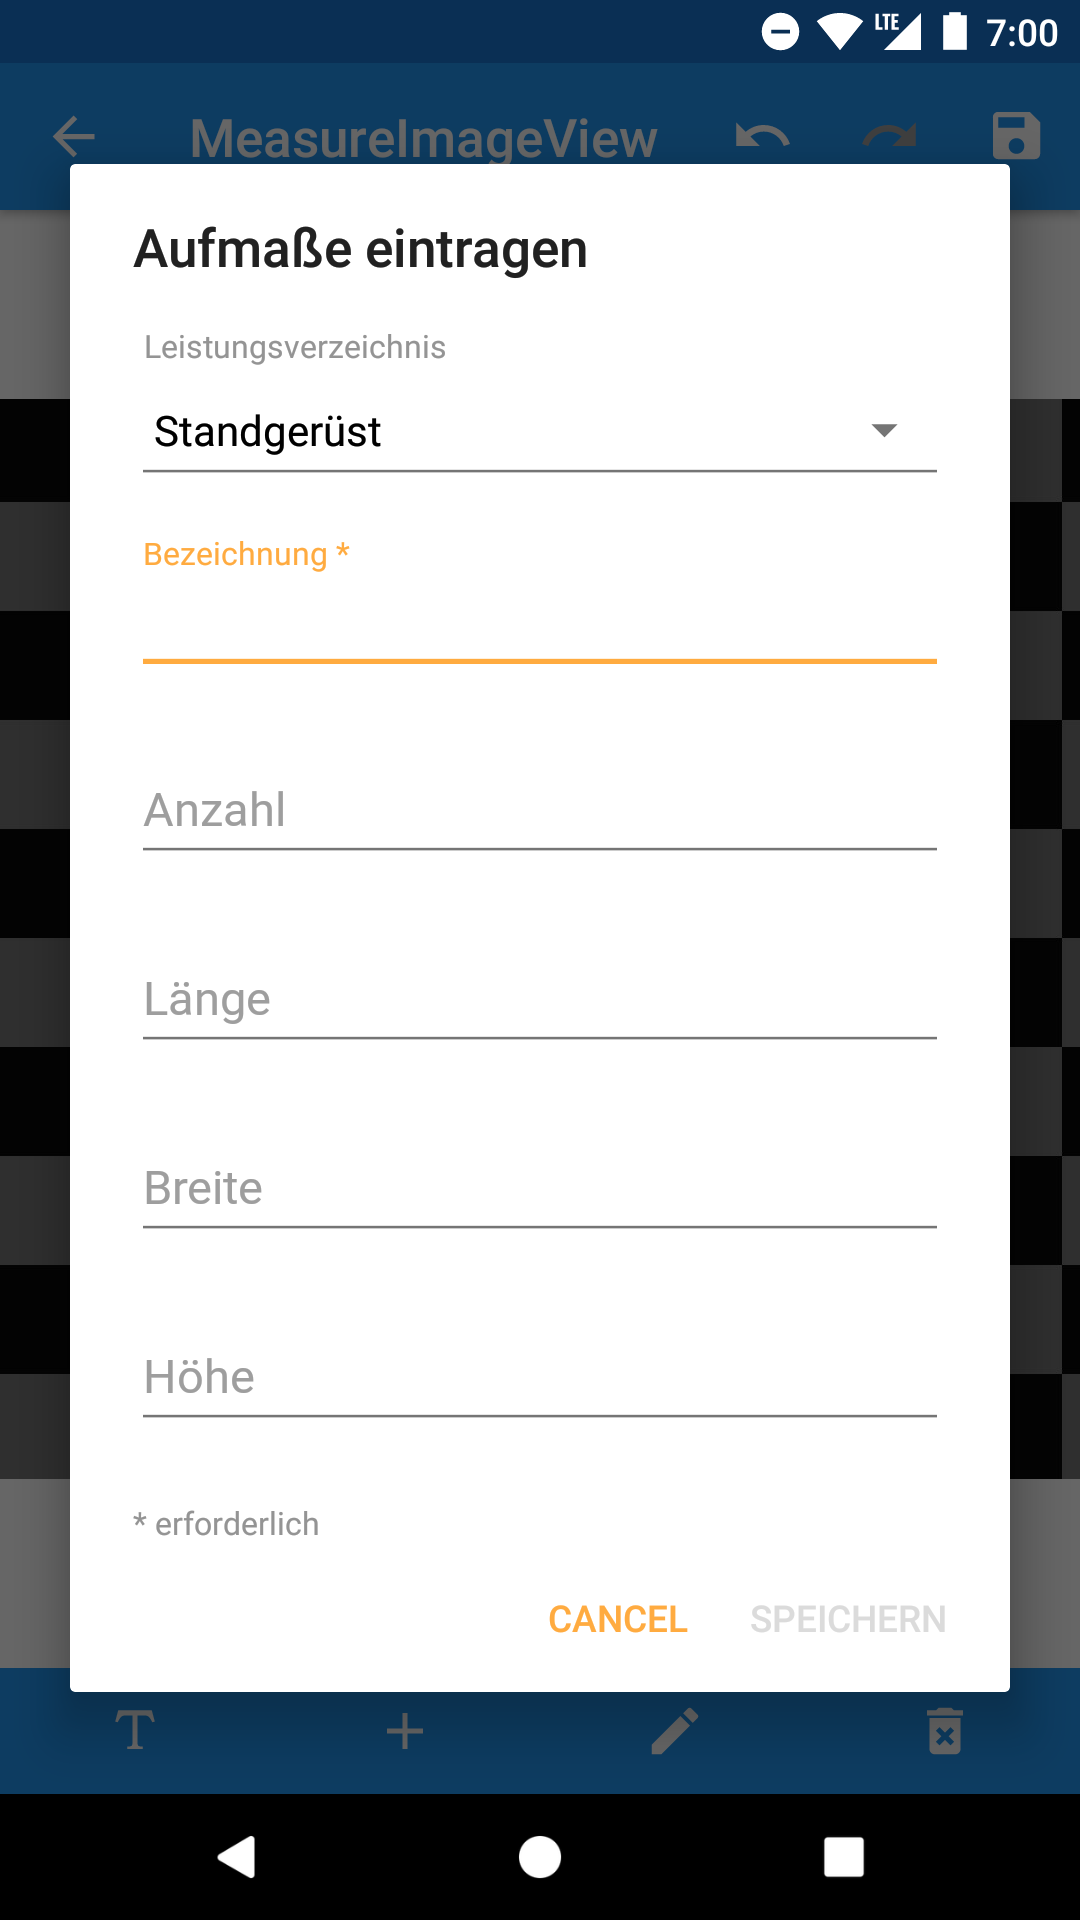
\includegraphics[keepaspectratio, width=0.4\textwidth]{prototype2/measure}
  \caption{Gerüsttyp-Dialog des zweiten Prototyps}
  \label{fig:dialog2}
\end{wrapfigure}

Im Zeichen-Modus (vgl. \autoref{fig:mode2}) kann per Klick auf das zweite Icon von links die gewünschte Form ausgewählt werden. 
Das Icon passt sich beim Ändern der Form an, und gibt so jederzeit Auskunft über die aktuell ausgewählte Zeichenform.
In \autoref{fig:mode2} ist bspw. zur Zeit die Linien-Form ausgewählt.
Im selben Modus kann beim Klick auf das dritte Icons (Farbpalette) die gewünschte Zeichenfarbe im Voraus konfiguriert werden. 
Hierzu öffnet sich, wie schon beim ersten Prototyp, ein modaler Farbauswahl-Dialog.
Auch dieses Icon passt sich dem Systemzustand an, und zeigt zu jeder Zeit die ausgewählte Farbe.
So ist in \autoref{fig:mode2} bspw. aktuell die Farbe Weiß ausgewählt.
Das vierte Icon (Mülleimer) ermöglicht im Zeichen- sowie im Text-Modus das Löschen der zuvor ausgewählten Form bzw. des markierten Textes. 
Hierbei wird der Nutzer nicht nach einer Bestätigung des Löschvorgangs gefragt, da unabsichtlich gelöschte Formen über die Undo-Funktion wiederhergestellt werden können. \\

Im Text-Modus kann beim Klick auf das zweite Icon von links (Plus-Zeichen) entweder eine ausgewählte Form mit einer Beschriftung versehen, oder mit einem Gerüsttyp verknüpft werden (siehe \autoref{fig:labelp2}).
Beim Hinzufügen einer Beschriftung öffnet sich ein modaler Eingabedialog, in den der Benutzer den gewünschten Text eintragen kann.
Entscheidet sich der Nutzer die ausgewählte Form mit einem Gerüsttyp zu verknüpfen, so öffnet sich der Gerüsttyp-Dialog (siehe \autoref{fig:dialog2}), der dem Nutzer über ein \emph{Dropdown} alle möglichen Gerüsttypen aus einem Leistungsverzeichnis zur Verfügung stellt.
Das dritte Icon von links (Stift) ermöglicht das Bearbeiten von bereits eingetragenen Messwerten und verknüpften Gerüsttypen.
Auch in diesem Modus sind die Icons nur dann auswählbar, wenn der aktuelle Systemzustand dies zulässt. 
So ist bspw. in \autoref{fig:mode2} keine Form ausgewählt und deshalb das Mülleimer-Icon nicht auswählbar. 
In \autoref{fig:labelp2} dagegen kann die ausgewählte Linie ohne Probleme gelöscht werden. \\

Für eine einfachere und nicht so fehleranfällige Benutzung auf Tablet-Geräten wurden sämtliche Größen mit Hilfe von dichteunabhängigen Pixeln modelliert, wie sie in den ``Android Developer Guides'' suggeriert werden.
So sind hierbei alle Größen der UI-Elemente in der Einheit \emph{dp} (``density-independent pixel'') angegeben, welche zur Laufzeit vom Android-System in normale Pixel (\emph{px}) umgewandelt werden.
Die genaue Umformung lautet dabei wie folgt:
\[
  px =  dp \times (\frac{dpi}{160}),
\]
wobei $dp$ für ``dots per inch'' steht.
Dies stellt sicher, dass alle Elemente unabhängig von der Bildschirmgröße gleich groß dargestellt werden. \\

Um die Lesbarkeit der eingetragenen Messwerte bei dunkleren Bildern zu verbessern, wurde die Textfarbe der Messwerte auf weiß geändert und zusätzlich wurden halbtransparente schwarze Rechtecke hinter den Text gelegt (siehe \autoref{fig:label2}).
Hierdurch soll vermieden werden, dass der Text auf dunkleren Bildern, wie bspw. in \autoref{fig:label1}, nicht gut lesbar ist.
\begin{figure}[h]
  \begin{subfigure}[t]{0.4\textwidth}
    \centering
    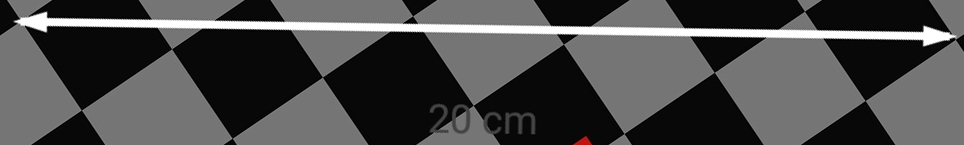
\includegraphics[keepaspectratio, width=\textwidth]{prototype2/label1}
    \caption{Eingetragener Messwert beim ersten Protoyp}
    \label{fig:label1}
  \end{subfigure}
  ~
  \begin{subfigure}[t]{0.4\textwidth}
    \centering
    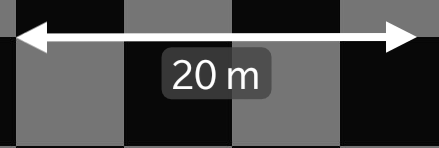
\includegraphics[keepaspectratio, width=\textwidth]{prototype2/label2}
    \caption{Eingetragener Messwert beim zweiten Prototyp}
    \label{fig:label2}
  \end{subfigure}
  \centering
  \caption{Vorher-Nachher-Vergleich: Darstellung der eingetragenen Messwerte}
  \label{fig:labels}
\end{figure}

Das Zuordnen von Gerüsttypen zu gezeichneten Formen (vgl. \autoref{fig:dialog2}) wurde mit Hilfe eines modalen Dialogs umgesetzt, der neben dem Gerüsttyp auch noch Textfelder für die verschiedenen Dimensionen des Gerüsts besitzt.
Hierdurch kann der Benutzer nicht nur den Gerüsttyp, sondern auch Maße des Gerüsts, welche im Bild aufgrund des Aufnahmewinkels eventuell nicht zu sehen sind, eintragen und in den Meta-Daten speichern.
Verknüpfte Formen zeigen mittels eines Indikators, ob und mit wie vielen Gerüsttypen sie verbunden sind.
Auf diese Weise soll der Benutzer die bereits verknüpften von den nicht-verknüpften Formen unterscheiden können. \\

Für das Schneiden und Rotieren von Bildern vor dem Annotieren wurde \emph{uCrop}\urlnote{https://github.com/Yalantis/uCrop}{03.01.2018}, eine dedizierte Android-Library, in das Projekt eingebunden.
\emph{uCrop} ist auf \emph{Github} als \emph{Open-Source} Projekt verfügbar und kann so den eigenen Bedürfnissen angepasst werden. 
Zudem unterstützt \emph{uCrop} alle Android-Geräte unabhängig vom Gerätehersteller ab der Android-Version \emph{Ice Cream Sandwich}. 
Dies entspricht laut der Verteilung der Android-Versionen auf allen Geräten mit Android OS im Zeitraum vom 5. bis 11. Dezember 2017 mehr als $99\%$ aller Geräte (vgl. \autoref{fig:versionchart}).
Zusätzlich zum Zuschneiden und Rotieren des Bildes bietet \emph{uCrop} auch das Ändern des Bildformates an (siehe \autoref{fig:ucrop}).
Hier kann der Nutzer auswählen, ob das Bild im originalen, ``1:1'', ``3:4'', ``3:2'' oder ``16:9'' Bildseitenverhältnis importiert werden soll.

\begin{figure}[h]
  \begin{subfigure}[t]{0.4\textwidth}
    \centering
    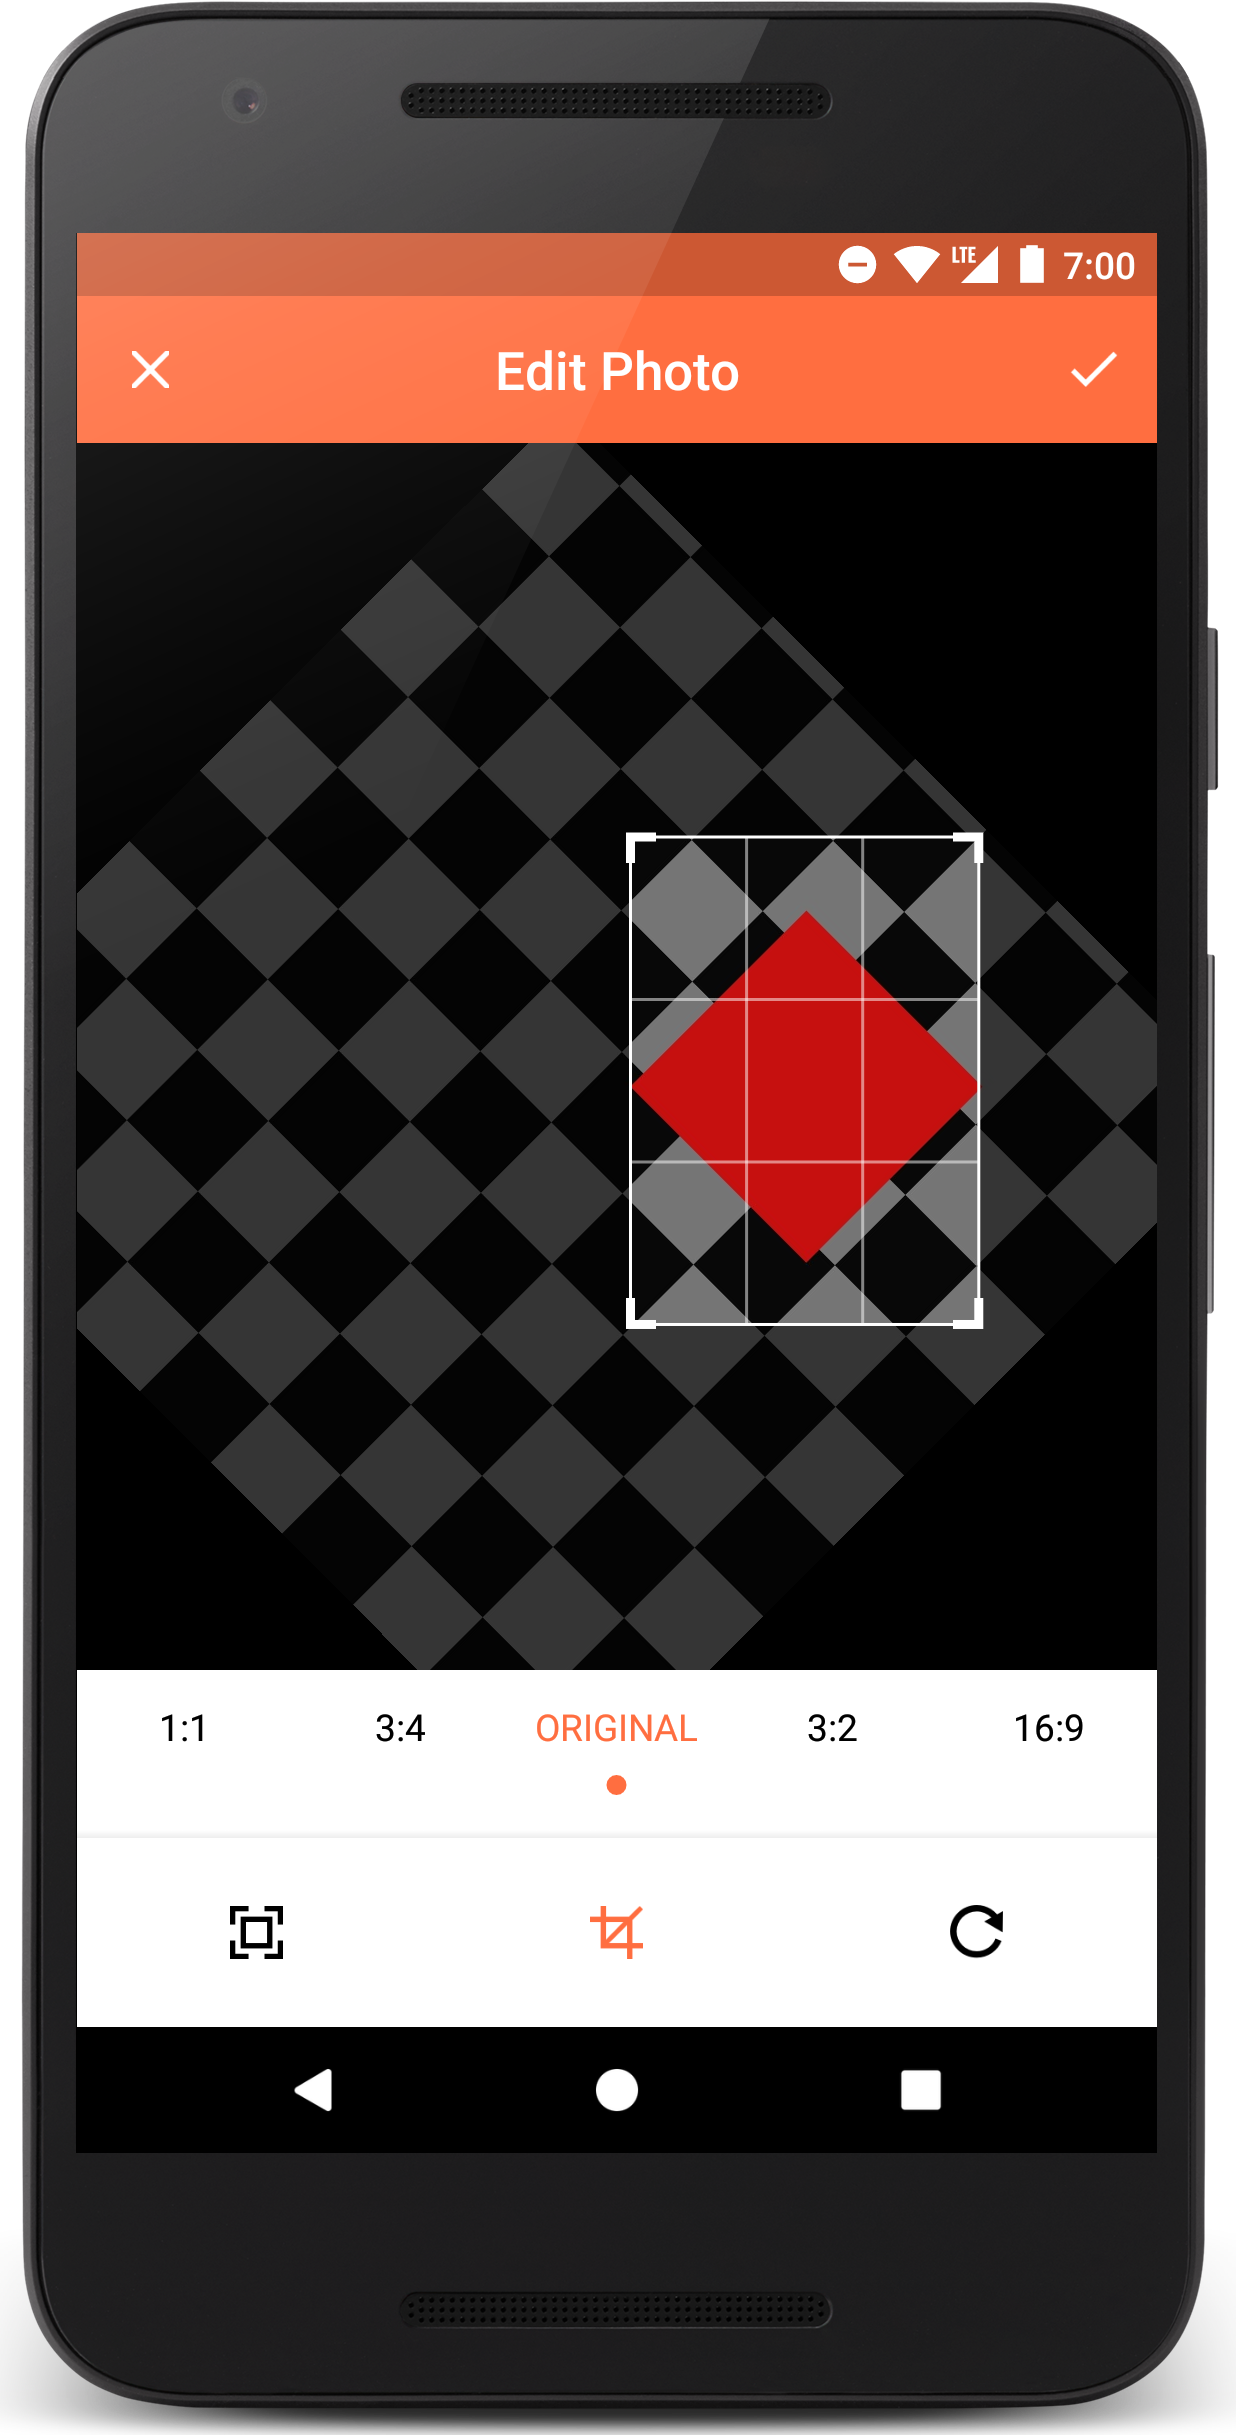
\includegraphics[keepaspectratio, width=\textwidth]{prototype2/ucrop}
    \caption{Rotation und Verkleinerung des Bildbereichs}
  \end{subfigure}
  ~
  \begin{subfigure}[t]{0.4\textwidth}
    \centering
    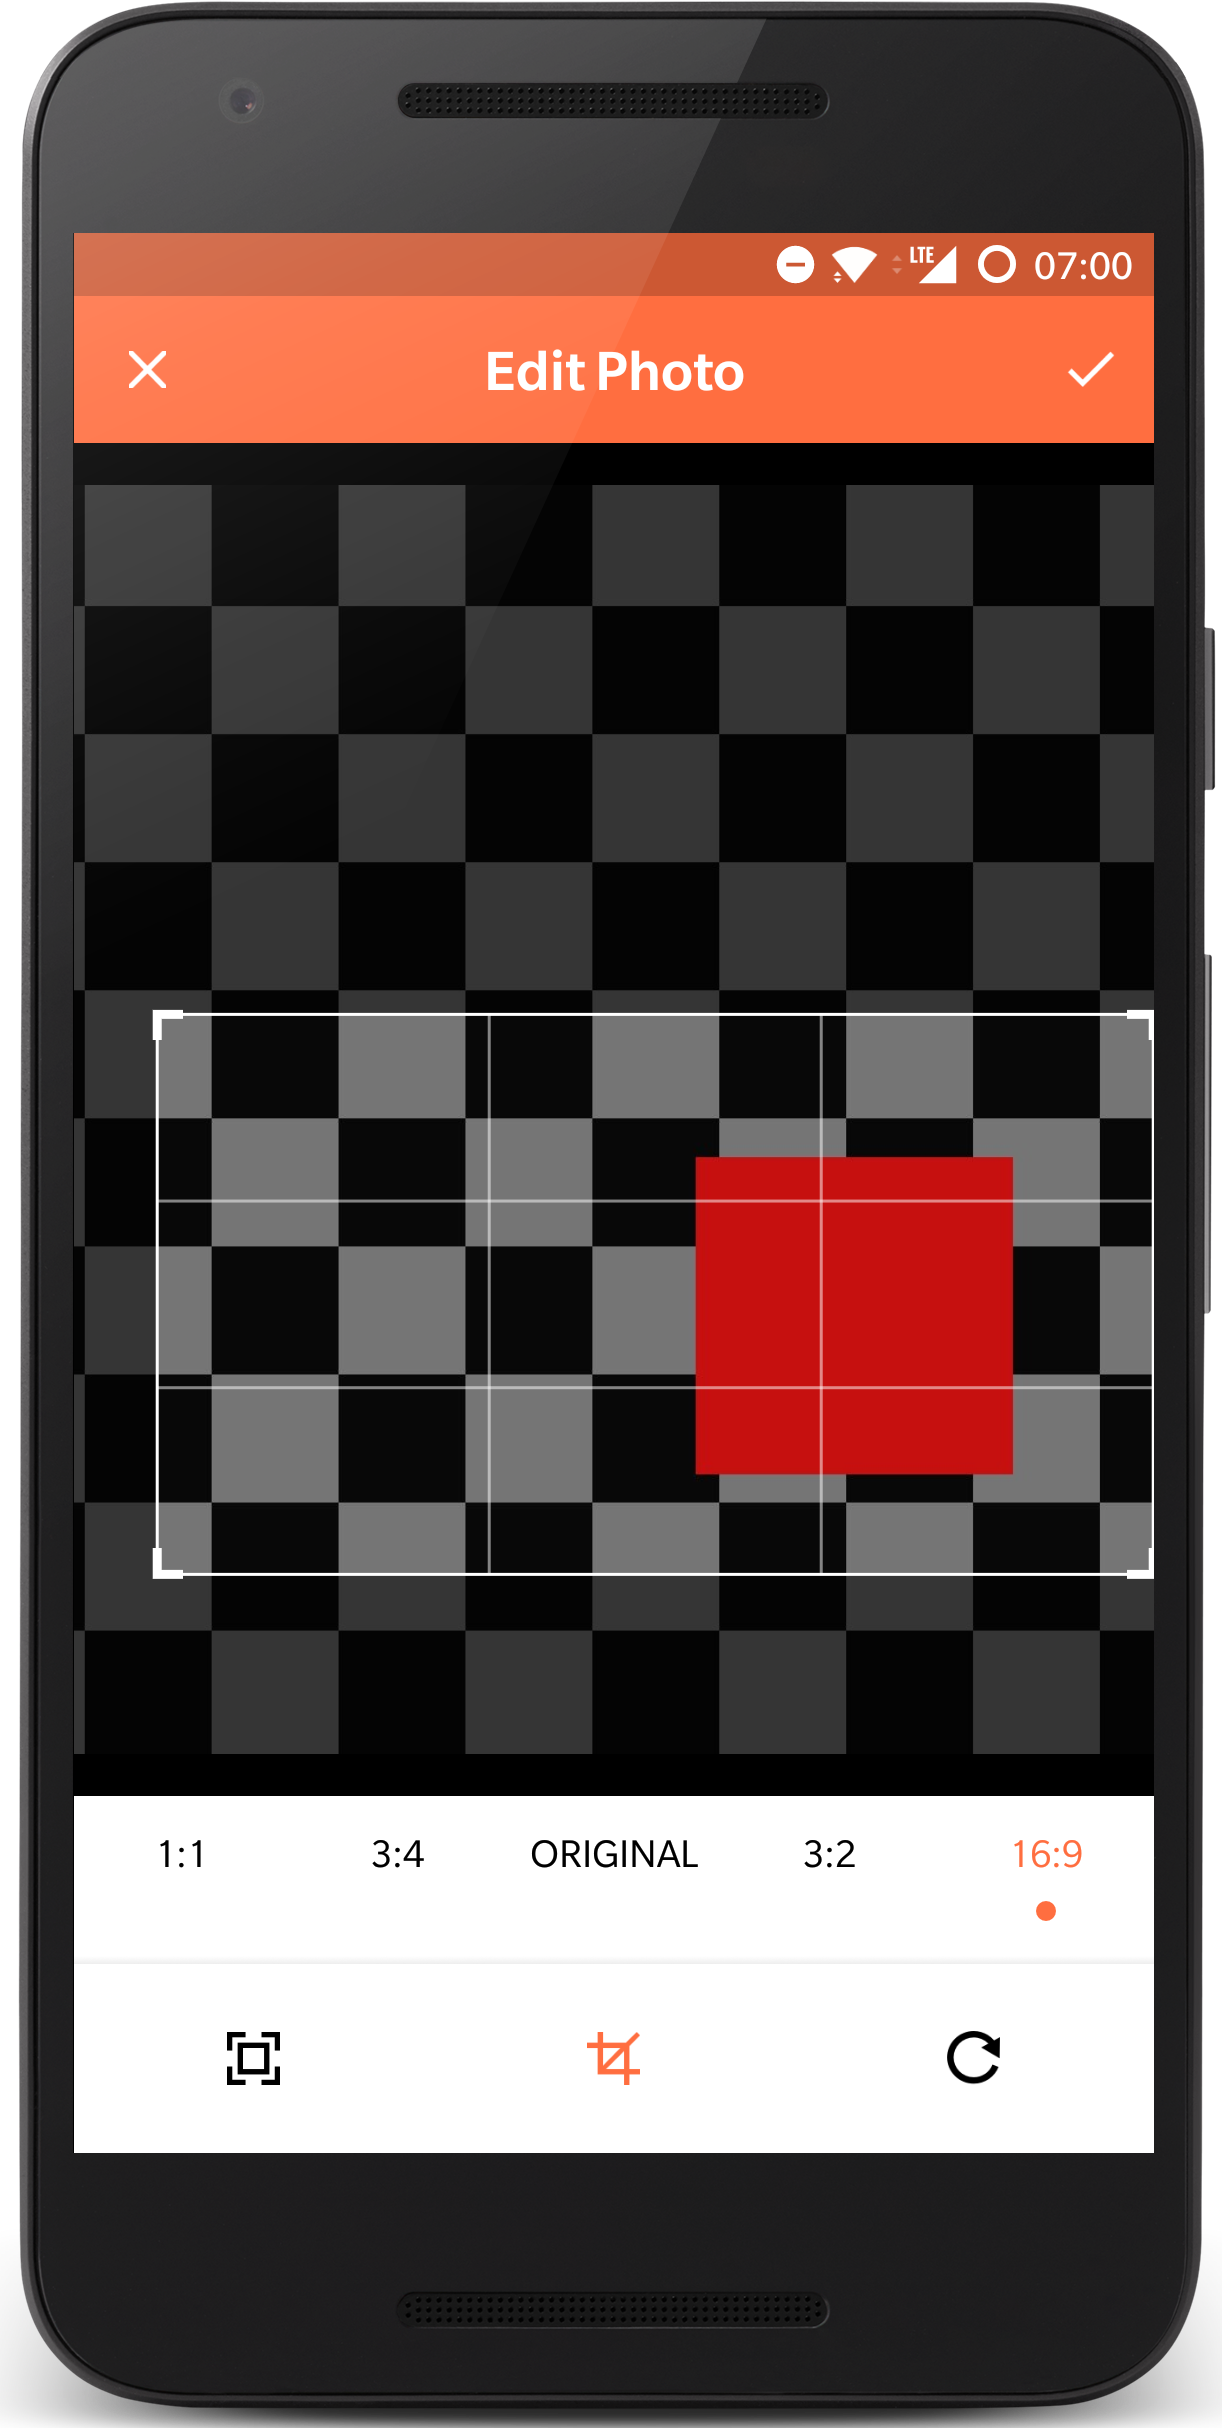
\includegraphics[keepaspectratio, width=\textwidth]{prototype2/ucrop2}
    \caption{Änderung des Bildseitenverhältnis auf ``16:9''}
  \end{subfigure}
  \centering
  \caption{\emph{uCrop}-Library zum Zuschneiden des Bildes im zweiten Prototyp}
  \label{fig:ucrop}
\end{figure}

\section{Testing}\label{sec:test2}
Der zweite Prototyp wurde sechs Tage, vom 3. bis zum 9. Januar 2018, von den beiden Testpersonen in ihren Arbeitsalltag integriert.
Das anschließende Feedback resultiert aus einem Gespräch mit beiden Testpersonen am 9. Januar. \\

Als deutlich positive Verbesserung wurde dabei von beiden Testpersonen die neue Statusleiste am unteren Bildschirmrand genannt.
Hierdurch sei ihnen die Benutzung der App um einiges leichter gefallen, als noch beim ersten Prototyp mit den \emph{Floating Action Buttons}. \\

Jedoch sei, so beide Tester, das initiale Einarbeiten in die App immer noch zu schwierig, und nicht intuitiv genug.
Hier wünsche man sich eine ``kleine Anleitung, die die App kurz beschreibt'' (Testperson 2) \\

Ein weiteres Problem, dass beim Testen des Prototyps aufgefallen ist, sei der Farbdialog.
Dieser sei nach Aussage von Testperson 1, zu fortgeschritten und biete eine Auswahl an Farben, die ``[...] der normale Gerüstbauer niemals verwenden wird'' (Testperson 1).
Hierbei wäre es laut Testperson 1 sinnvoller, den Benutzer ``[...] nicht mit so vielen Auswahlmöglichkeiten zu überschütten [...]'', sondern die populärsten Farben direkt auswählbar zu machen. \\

Außerdem wurde sich neben einem einfacheren Farbdialog eine Funktion gewünscht, Freitexte in das Bild eintragen zu können. 
Dies sei laut der Aussage beider Tester eine wichtige Funktion, da es bisher keine Möglichkeit gibt, weitere Notizen oder Anmerkungen im Bild zu hinterlegen \\

Zudem kam der Wunsch nach einer weiteren Form, nämlich einer Linien mit nur einer Pfeilspitze, auf.
Dies sei, so beide Testpersonen, wichtig, um Längen, die auf dem Bild nur einen Startpunkt haben, und in die Tiefe offen sind, zu kennzeichnen oder bestimmte Details hervorzuheben. \\

Des Weiteren seien verlinkte Gerüsttypen an Formen nicht intuitiv durch den in diesem Prototyp eingeführten Indikator erkennbar.
Hierzu fügten beide Testpersonen hinzu, dass die Eingabefelder zum Eintragen der Messwerte im Gerüsttyp-Dialog ``[...] durchaus sinnvoll [...]'' (Testperson 1) seien, in der Praxis jedoch daran scheitern würde, dass sich Messwerte zuerst gemerkt werden müssen, bevor sie im Dialog eingegeben werden können.
Dies habe sich besonders dann als Problem herausgestellt, wenn mehr als ein Messwerte zugleich eingetragen werden sollten. \\

Zusammenfassend lässt sich festhalten, dass sich in dieser Testphase sowohl neue Usability-Probleme, als auch neue Anwenderwünsche identifizieren lassen haben.
Diese Ergebnisse sollen in einer weiteren Iteration des \hcdp{} im nächsten Kapitel genauer untersucht werden.

\chapter{Dritte Iteration - Initiale Hilfestellung}\label{chap:pro3}
Die beim Testen des zweiten Prototyps in \autoref{sec:test2} identifizierten Probleme sollen nun in einer dritten Iteration des \hcdp{} gelöst werden.
Hierzu werden, wie schon im vorherigen Abschnitt, die vier Phasen des Zyklus ein weiteres Mal durchlaufen.
Das Ziel dieses Kapitels ist es, durch die Entwicklung eines dritten Prototyps die Usability-Probleme aus dem Zweiten zu lösen, und die Anwenderwünsche aus dem vorherigen Kapitel umzusetzen.

\section{Observation}\label{sec:obs3}
Um auch in diesem Abschnitt einen Überblick über die gesammelten Test-Ergebnisse aus \autoref{sec:test2} zu bekommen, werden diese im Nachfolgenden zur Übersicht aufgelistet und anschließend weiter evaluiert:

\begin{itemize}
  \item Hilfestellung beim initialen Start der App unzureichend
  \item Auswahlmöglichkeiten im Farbdialog zu fortgeschrittenen
  \item Gerüsttyp-Indikator nicht intuitiv als solcher erkennbar
  \item Kognitive Last beim Eintragen der Messwerte im Gerüsttyp-Dialog zu hoch
  \item Anwenderwunsch: Einführen einer Freitext-Form
  \item Anwenderwunsch: Einführen einer Pfeil-Form 
\end{itemize}

\noindent
Die Testergebnisse zeigen, dass beide Testpersonen in \autoref{sec:test2} Nutzungsprobleme aufgrund einer unzureichenden Hilfestellung beim initialen Start der App gehabt haben.
Daher müssen Funktionen der App durch ``Trial and Error'' erkundet werden.
Dies erzeugt nicht nur einen negativen ersten Eindruck beim Nutzer, sondern potenziert das Auftreten von Situationen, in denen Fehler enstehen können.
Besonders diese beiden Punkte führen schnell zu einem negativen Anwendererlebnis der App, und erschweren somit bereits zu Beginn die Nutzung der App.
(Nielsen~\autoref{itm:N5} \& \autoref{itm:N13}) \\

Die zu fortgeschrittenen Auswahlmöglichkeiten im Farbdialog sind ein weiteres Usability-Problem, das sich während der Testphase in \autoref{sec:test2} gezeigt hat.
Durch die Verwendung eines Farbkreises, der das Auswählen einer beliebigen Farbe und der dazugehörigen Transparenz ermöglicht, zeigen sich beide Testpersonen überfordert.
Diese vielen Auswahlmöglichkeiten übertreffen das Ziel des Benutzers, der nur schnell und unkompliziert eine Farbe auszuwählen möchte.
(Nielsen~\autoref{itm:N12}) \\

Außerdem wird aus den Testergebnissen ersichtlich, dass der verwendete Indikator für die verlinkten Gerüsttypen nicht intuitiv als solcher erkennbar ist.
Die Benutzung einer einzelnen Zahl als Indikator für die Anzahl der verknüpften Gerüste zu einer Form hat nicht genug Wiedererkennungswert, um mit den Gerüsttypen assoziiert zu werden.
Hier fehlt ein wiedererkennbares Icon, welches dem Benutzer den Kontext des Indikators intuitiv vermittelt.
(Nielsen~\autoref{itm:N6}) \\

Zudem belasten die Eingabefelder im Gerüsttyp-Dialog die kognitiven Fähigkeiten der Testpersonen zu sehr.
Da die Eingabefelder keinerlei Vorschläge für die einzutragenden Werte bieten, müssen die Nutzer sich die Messwerte merken, welche sie anschließend in den Dialog eintragen wollen.
Dies führt im schlimmsten Fall dazu, dass mehrfach zwischen Dialog und Bild gewechselt werden muss, um alle Messwerte in den Dialog eintragen zu können.
Weil Dialoge unter Android standardmäßig nicht minimiert, und zu einem späteren Zeitpunkt wieder angezeigt werden können, ohne dass eingetragenen Informationen verloren gehen, muss der Benutzer alle zuvor eingetragenen Daten beim Schließen und wieder Öffnen des Dialogs erneut eingeben.
(Nielsen~\autoref{itm:N11}) \\

Zusätzlich zu den Usability-Problemen des zweiten Prototyps, die sich in \autoref{sec:test2} gezeigt haben, gab es Wünsche für neue Funktionen, die regelmäßig im Arbeitsalltag der Testpersonen gebraucht werden.
So soll die App um zwei neue Formen, der Freitext- und Pfeil-Form, erweitert werden.
Die Freitext-Form soll dem Nutzer ermöglichen, beliebige Texte auf das Bild zu schreiben, ohne zuvor eine Form zeichnen zu müssen. 
Durch die Pfeil-Form sollen Längen, die sich mit Hilfe der Linien-Form nicht gut abbilden lassen, dargestellt werden. \\

\section{Idea Generation}\label{sec:idea3}
Um dem Benutzer beim Start der App einen Überblick über die beiden Modi und den darin enthaltenen Funktionen zu geben, soll eine Hilfestellung beim initialen Start der App angezeigt werden.
Die \mg{} suggerieren zur Umsetzung eines solchen ``Onboarding''-Prozesses\urlnote{https://material.io/guidelines/growth-communications/onboarding.html\#onboarding-onboarding-models} drei verschiedene Ansätze (vgl. \autoref{fig:onboarding}). \\

\begin{figure}[h]
  \centering
  \begin{subfigure}[t]{0.3\textwidth}
    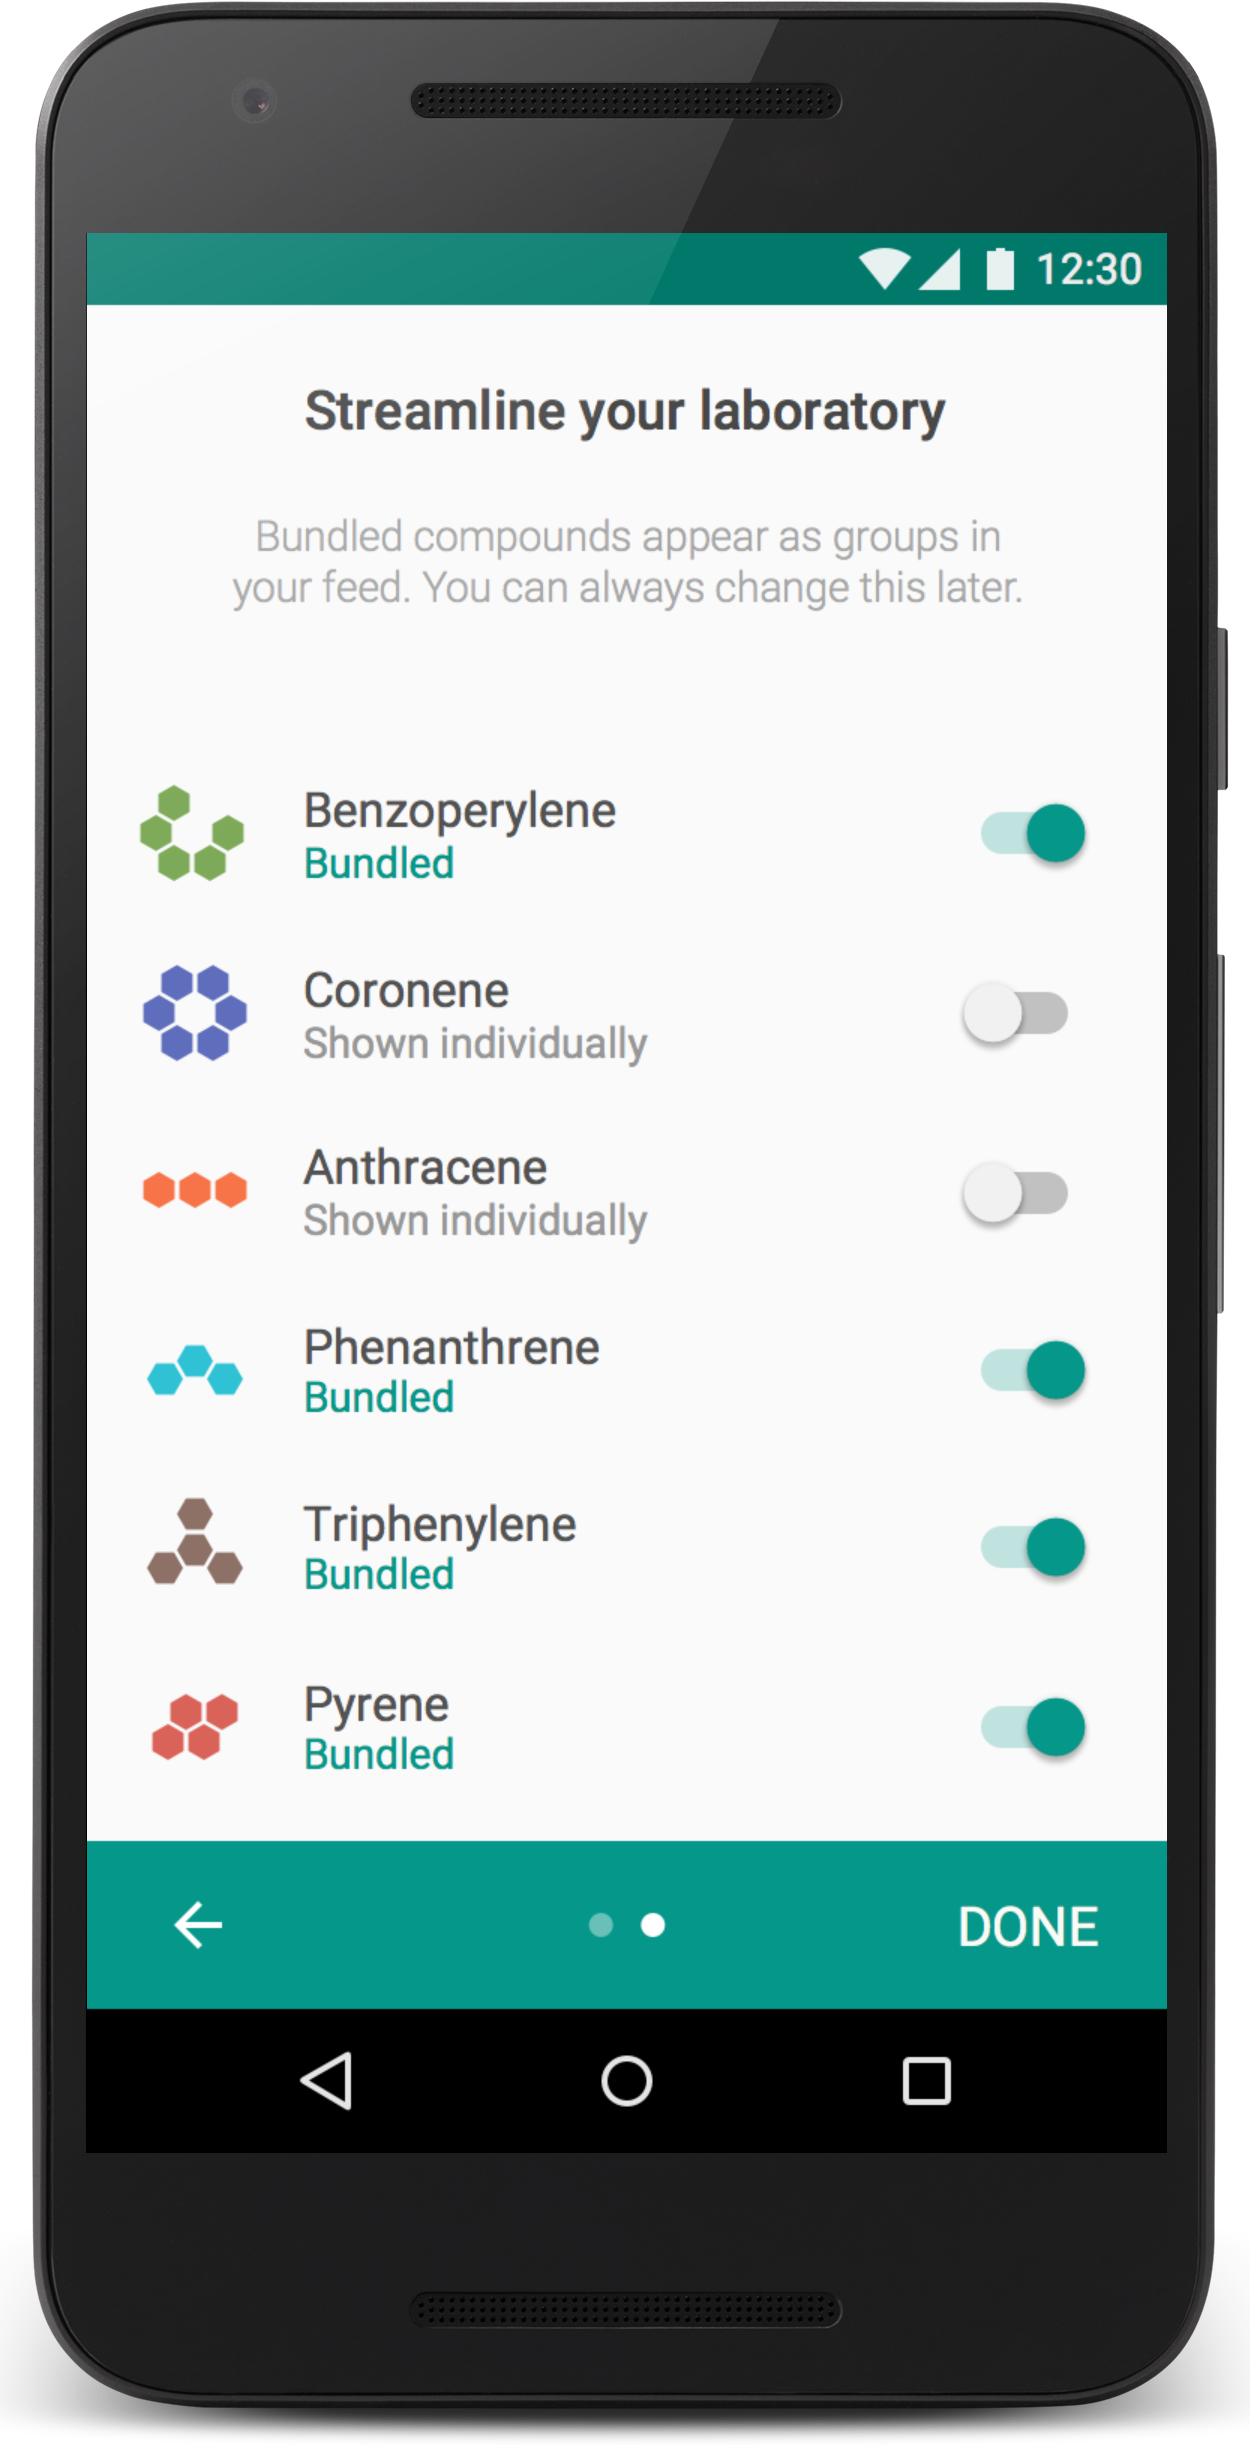
\includegraphics[keepaspectratio, width=\textwidth]{prototype3/selfselect}
    \caption{Selft-Select}
    \label{fig:selfselect}
  \end{subfigure}
  \begin{subfigure}[t]{0.3\textwidth}
    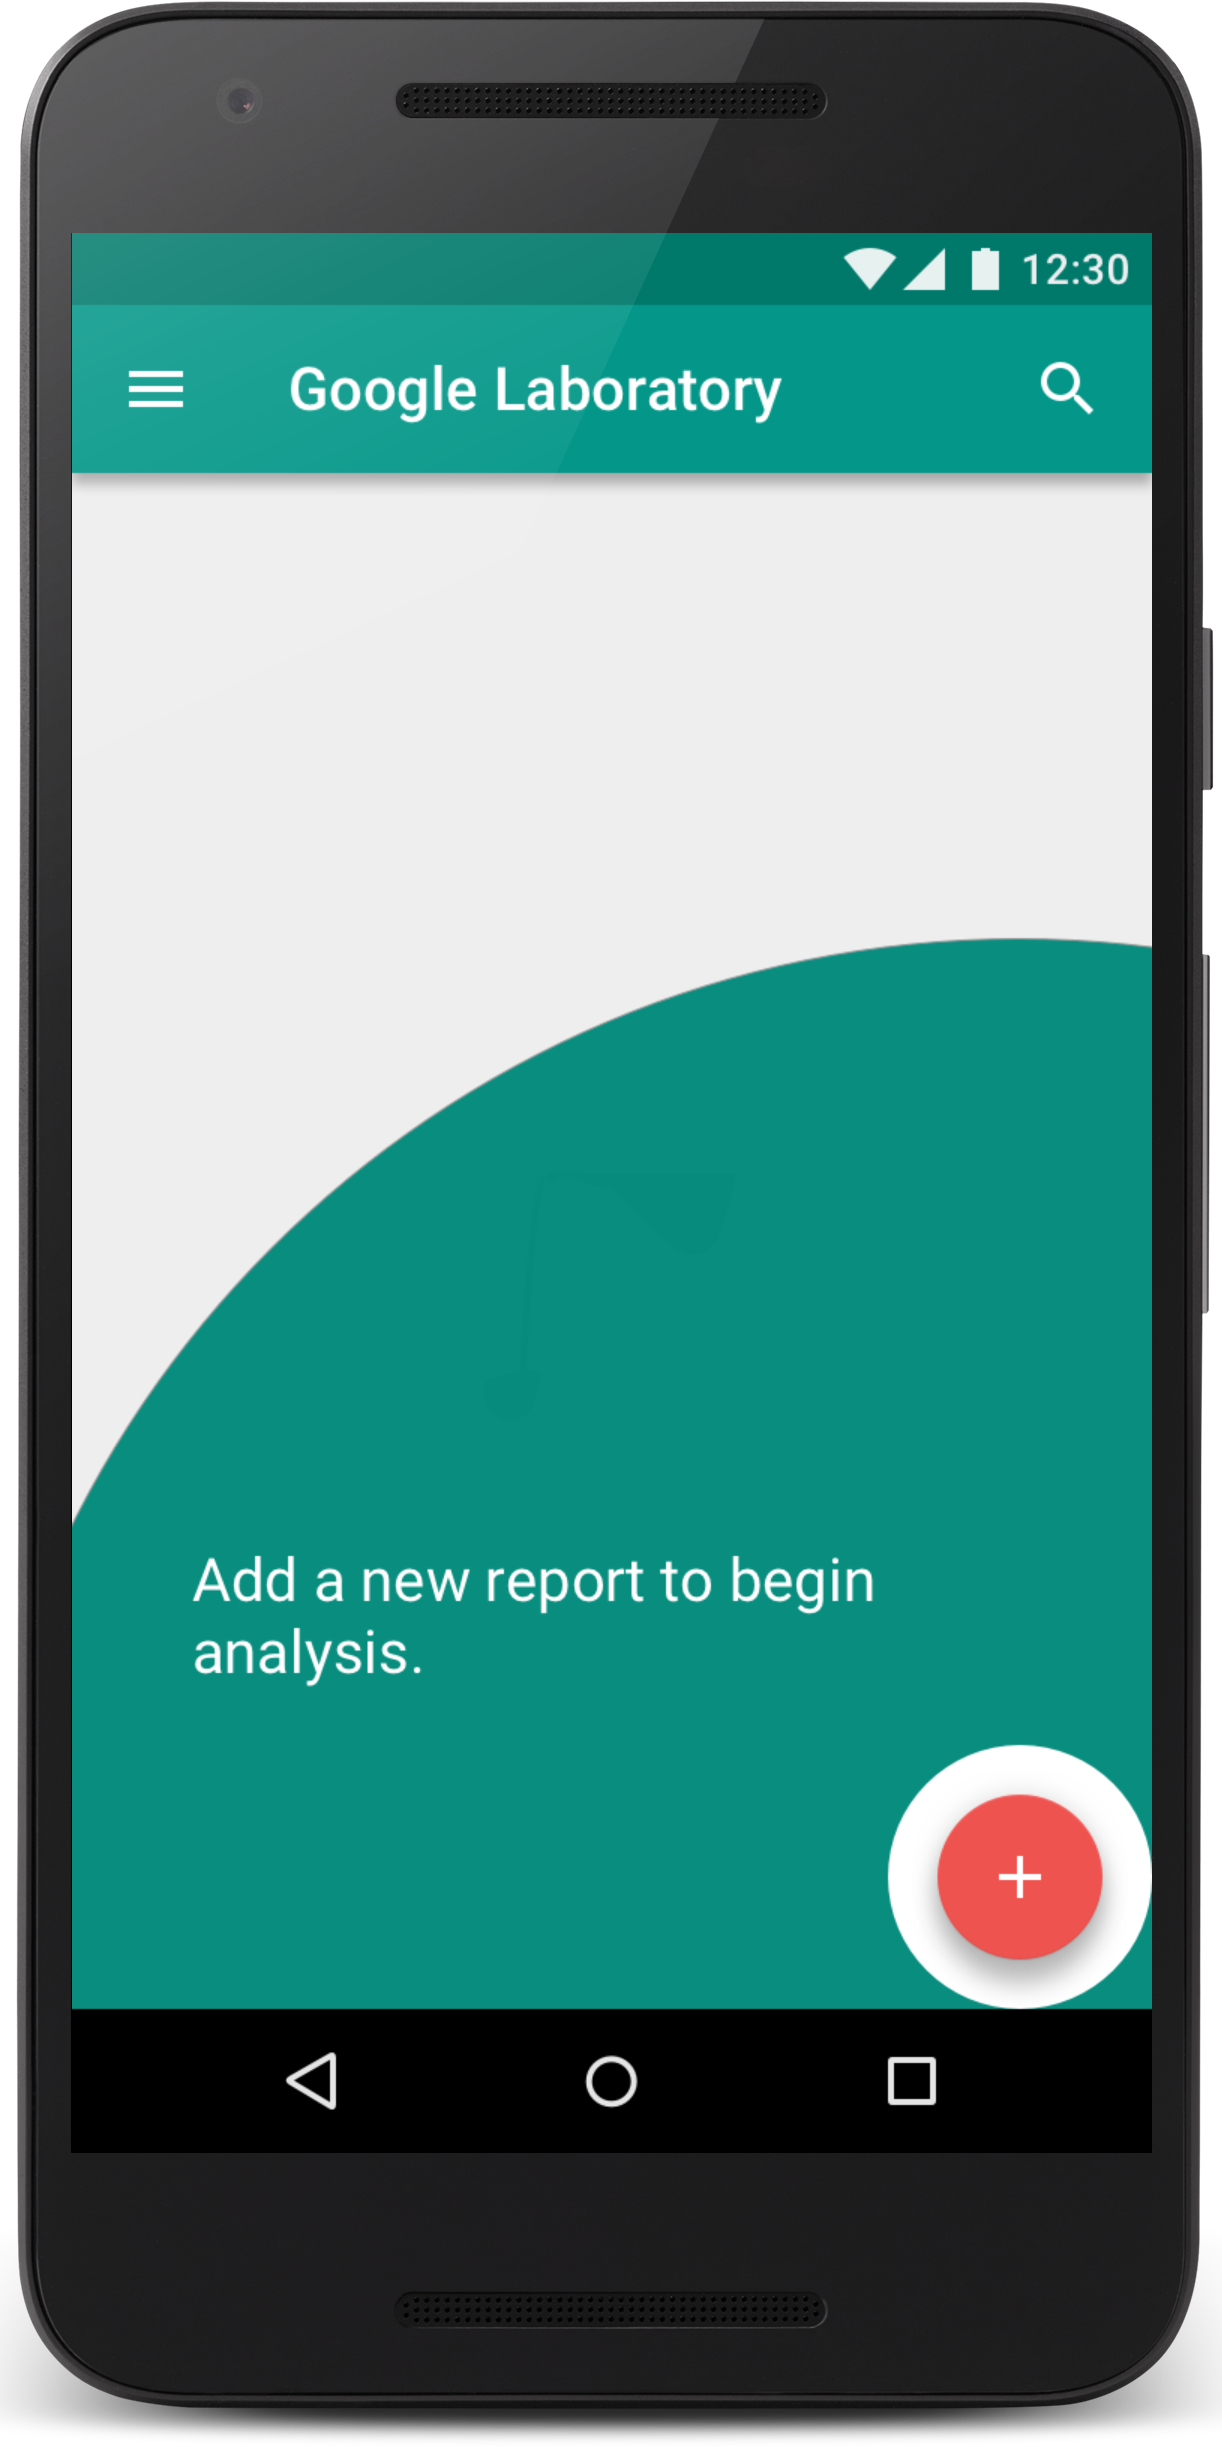
\includegraphics[keepaspectratio, width=\textwidth]{prototype3/quickstart}
    \caption{Quickstart}
    \label{fig:quickstart}
  \end{subfigure}
  \begin{subfigure}[t]{0.3\textwidth}
    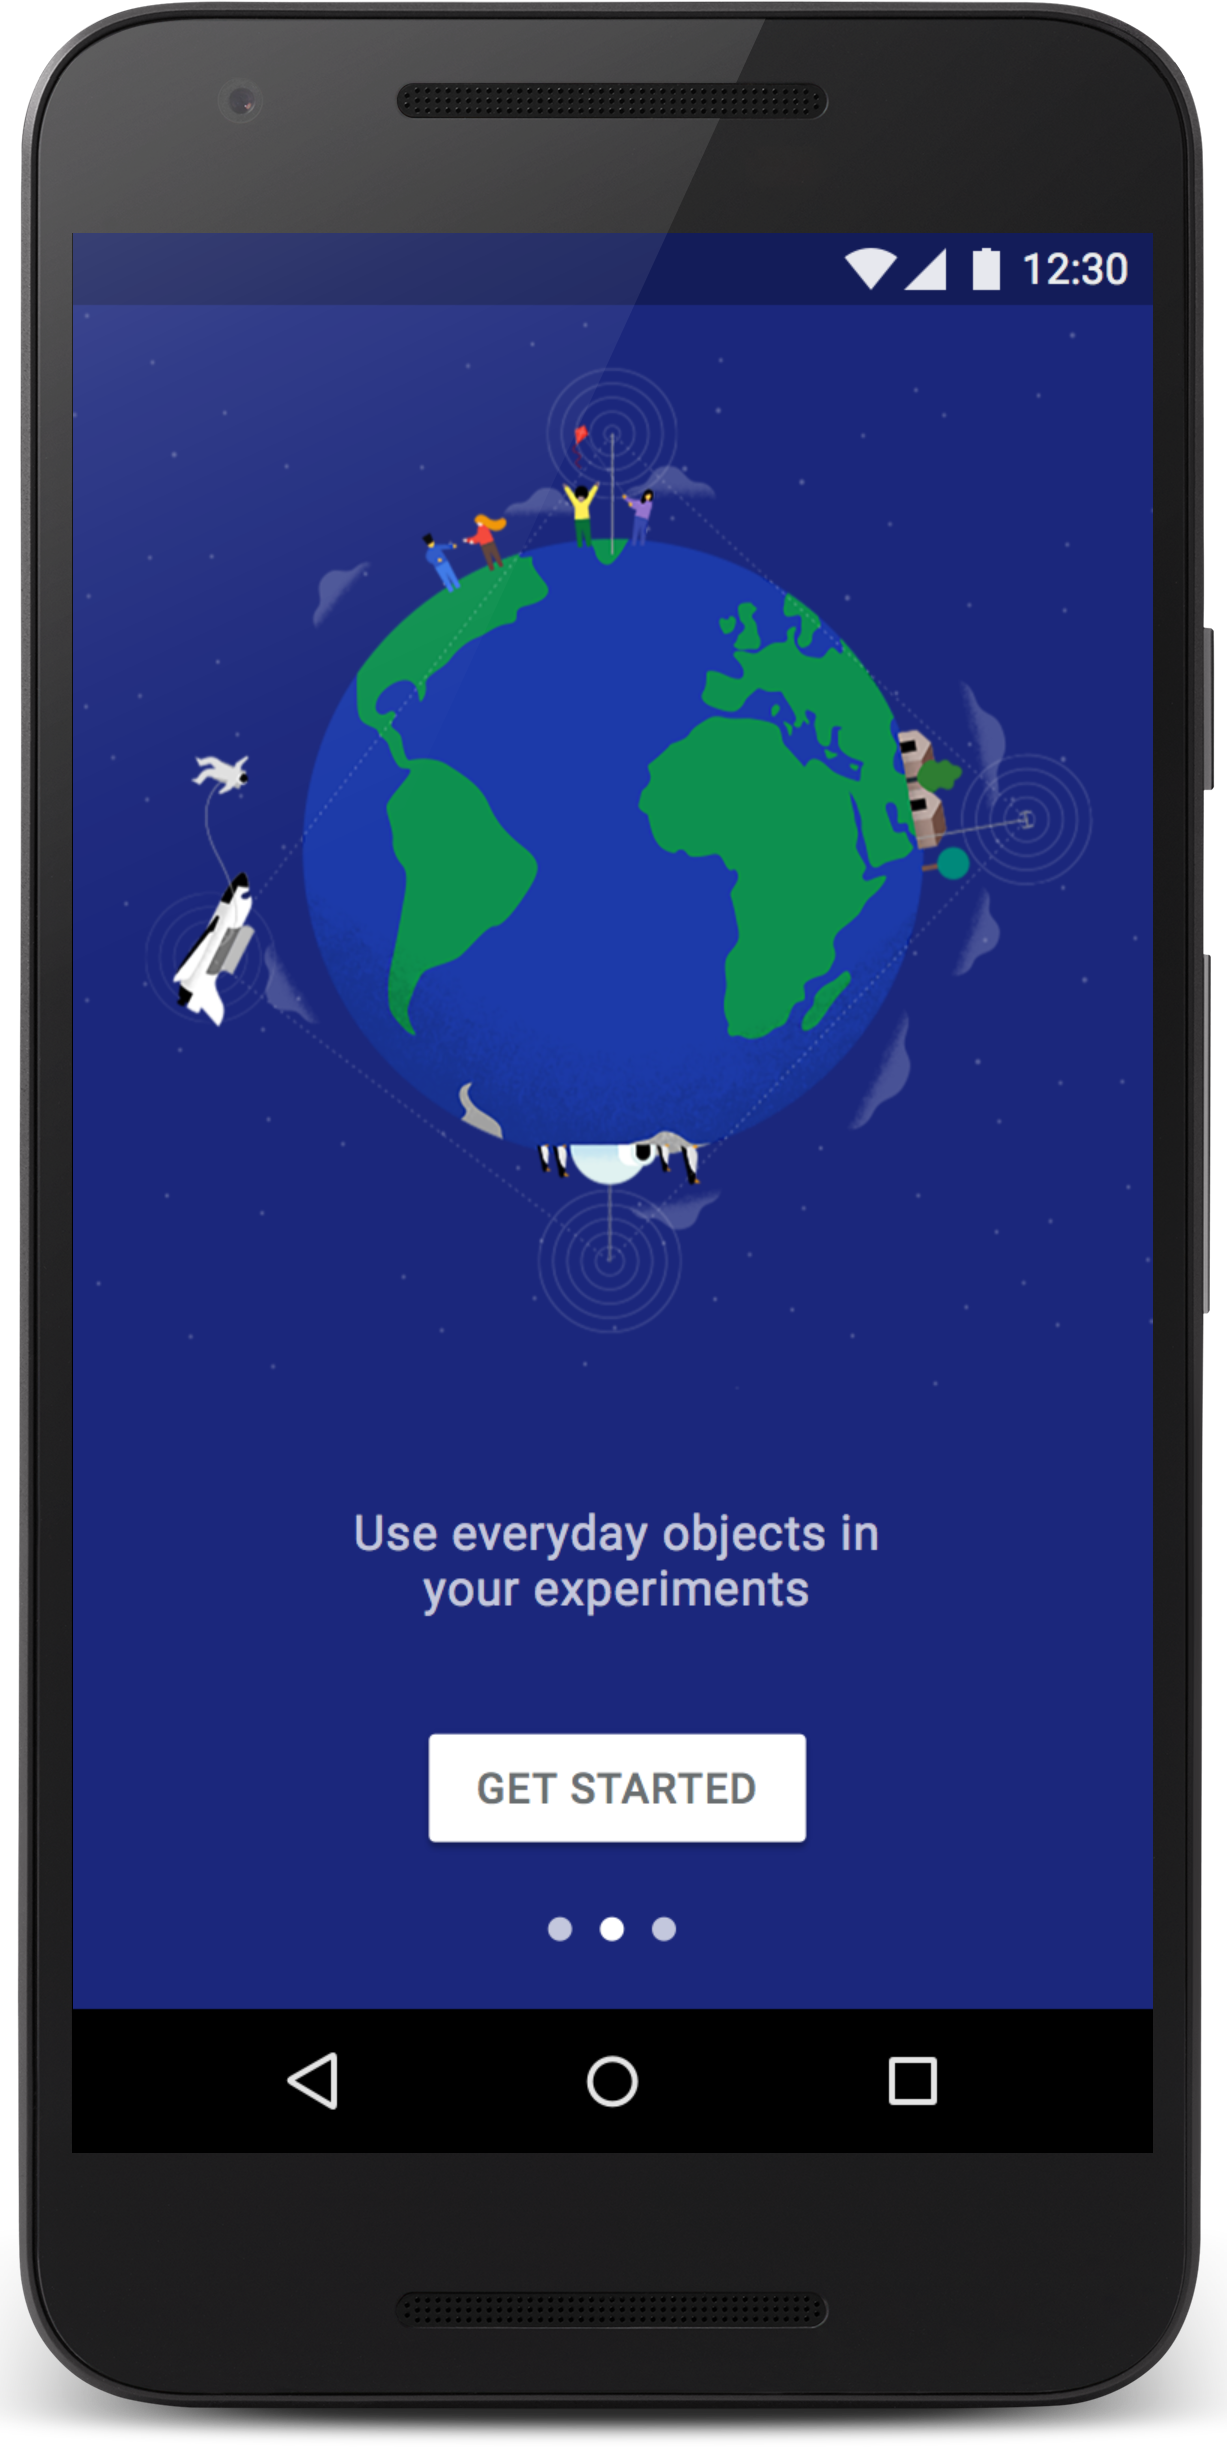
\includegraphics[keepaspectratio, width=\textwidth]{prototype3/userbenefits}
    \caption{Top User Benefits}
    \label{fig:benefits}
  \end{subfigure}
  \caption{Die drei verschiedenen ``Onboarding''-Ansätze nach den \mg{}}
  \label{fig:onboarding}
\end{figure}

Zu den drei ``Onboarding''-Ansätzen werden auch die jeweiligen ``Use-Cases'' angegeben, für die sich die Umsetzungsmöglichkeiten jeweils am Besten eignen \citep[Abschnitt ``Usage'']{Onboarding}.
So biete sich bspw. die \emph{Self-Select}-Variante (siehe \autoref{fig:selfselect}) dann an, wenn der Nutzer beim initialen Start der App bereits diverse Einstellungen konfigurieren muss.
Die \emph{Quickstart}-Variante (siehe \autoref{fig:quickstart}) solle, so die \mg{}, dann genutzt werden, wenn bereits identifiziert werden konnte, welche Funktionen der App besonders hervorgehoben werden soll.
Diese Funktion solle dem Nutzer dann beim initialen Start der App vorgestellt werden, und so als ``Call for action'' dienen.
Die Variante des \emph{Top User Benefits} (siehe \autoref{fig:benefits}) könne nach den \mg{} am besten dann sinnvoll eingesetzt werden, wenn neue Funktionalität oder große Änderungen der Benutzeroberfläche angekündigt werden sollen. \\

Damit der Farbdialog den Nutzer nicht mehr mit zu vielen Anpassungsmöglichkeiten überfordert, sollen diese auf ein Minimum reduziert werden.
So kann der Dialog bspw. so verändert werden, dass er nur eine Palette der häufigst genutzten Farben anzeigt, und auf die Einstellungsmöglichkeit der Transparenz ganz verzichtet.
Um die volle Breite des Farbkreises nicht zu verlieren, bietet es sich an, den fortgeschrittenen Modus, wie er im zweiten Prototyp standardmäßig angezeigt wird, über einen Button im Dialog zugänglich zu machen.
So kann der erfahrene Nutzer, falls er keine Farbe der Standardpalette benutzen möchte, über den fortgeschrittenen Modus eine beliebige Farbe und deren Transparenz auswählen. \\

Die Wiedererkennbarkeit des Gerüsttyp-Indikators könnte durch die Benutzung eines Icons neben der Indikator-Zahl verbessert werden.
Alternativ bietet es sich an, einen weiteren Text zum Indikator hinzuzufügen, der verdeutlicht, dass es sich bei der Indikator-Zahl um die Anzahl der verknüpften Gerüsttypen handelt.
Hierbei muss jedoch bei der praktischen Umsetzung darauf geachtet werden, dass nur eine begrenzte Menge Text auf dem Bildschirm gleichzeitig anzeigen werden sollte, bevor dieser zu unübersichtlich wird. \\

Um die kognitive Last der Nutzer beim Eintragen der Messwerte im Gerüsttyp-Dialog zu minimieren, bietet sich die Verwendung von Vorschlägen in den Eingabefeldern an.
Diese Vorschläge können dann z.B. aus den bereits hinterlegten Messwerten der jeweiligen Form stammen.
So hat der Nutzer zum Beispiel bei der Verlinkung einer Rechtecks-Form zu einem Gerüsttyp die Möglichkeit aus bis zu vier verschiedenen Vorschlägen (vier Kanten) auszuwählen.

Sowohl die Freitext- als auch die Pfeil-Form kann als Unterklasse der bestehenden abstrakten Oberklasse \emph{MeasureShape} modelliert werden.
Wichtig bei der Freitext-Form wird es sein, einen geeigneten Text-Hintergrund zu verwenden, damit der Text auch auf dunkleren Bildern ohne Anstrengung lesbar ist.
Hierzu bietet es sich an, die Ergebnisse aus \autoref{sec:idea2} bezüglich der Erkennbarkeit von eingetragenen Messwerten wiederzuverwenden.

\section{Prototyping}
Der dritte Prototyp wurde am 16. Januar 2018 in die bestehende Android-App eingebunden.
Bei der Implementierung dieses Prototyps wurde versucht alle in \autoref{sec:idea3} genannten Ideen zur Lösung der in \autoref{sec:obs3} identifizierten Probleme umzusetzen. \\

So wurde von den drei verschiedenen Ansatzmöglichkeiten zur Umsetzung des ``Onboarding''-Prozesses die Variante des \emph{Quickstarts} gewählt, da der ``Use-Case'' dieser am besten auf den Prototyp zutrifft.
Umgesetzt wurde die \emph{Quickstart} Variante mit Hilfe sogenannter \emph{Tap targets}\urlnote{https://material.io/guidelines/growth-communications/feature-discovery.html\#feature-discovery-design}.
Hiervon wurden insgesamt drei in den Prototyp integriert, welche jeweils an einer anderen Stelle dem Nutzer angezeigt werden (siehe \autoref{fig:taptargets}).
Ein \emph{Tap target} wird beim initialen Start der App angezeigt, und gibt dem Nutzer eine kurze Hilfestellung zu der \emph{Bottom bar} und dem damit verbundenen Zeichen- und Text-Modus (siehe \autoref{fig:helpmode}).
Die anderen beiden \emph{Tap targets} werden jeweils beim ersten Wechsel in den Text- bzw. Zeichen-Modus angezeigt, und beschreiben, welche Aktionen in dem jeweiligen Modus durchführbar sind (vgl. \autoref{fig:helpdraw} \& \autoref{fig:helptext}).
Die erklärenden Texte und auch die Position der einzelnen \emph{Tap targets} wurde so gewählt, dass der Nutzer die wichtigsten UI-Elemente der App fokussiert und über einen kurzen, aber präzisen Text alle wichtigen Informationen zur Benutzung dieser erhält. \\

\begin{figure}[h]
  \centering
  \begin{subfigure}[t]{0.3\textwidth}
    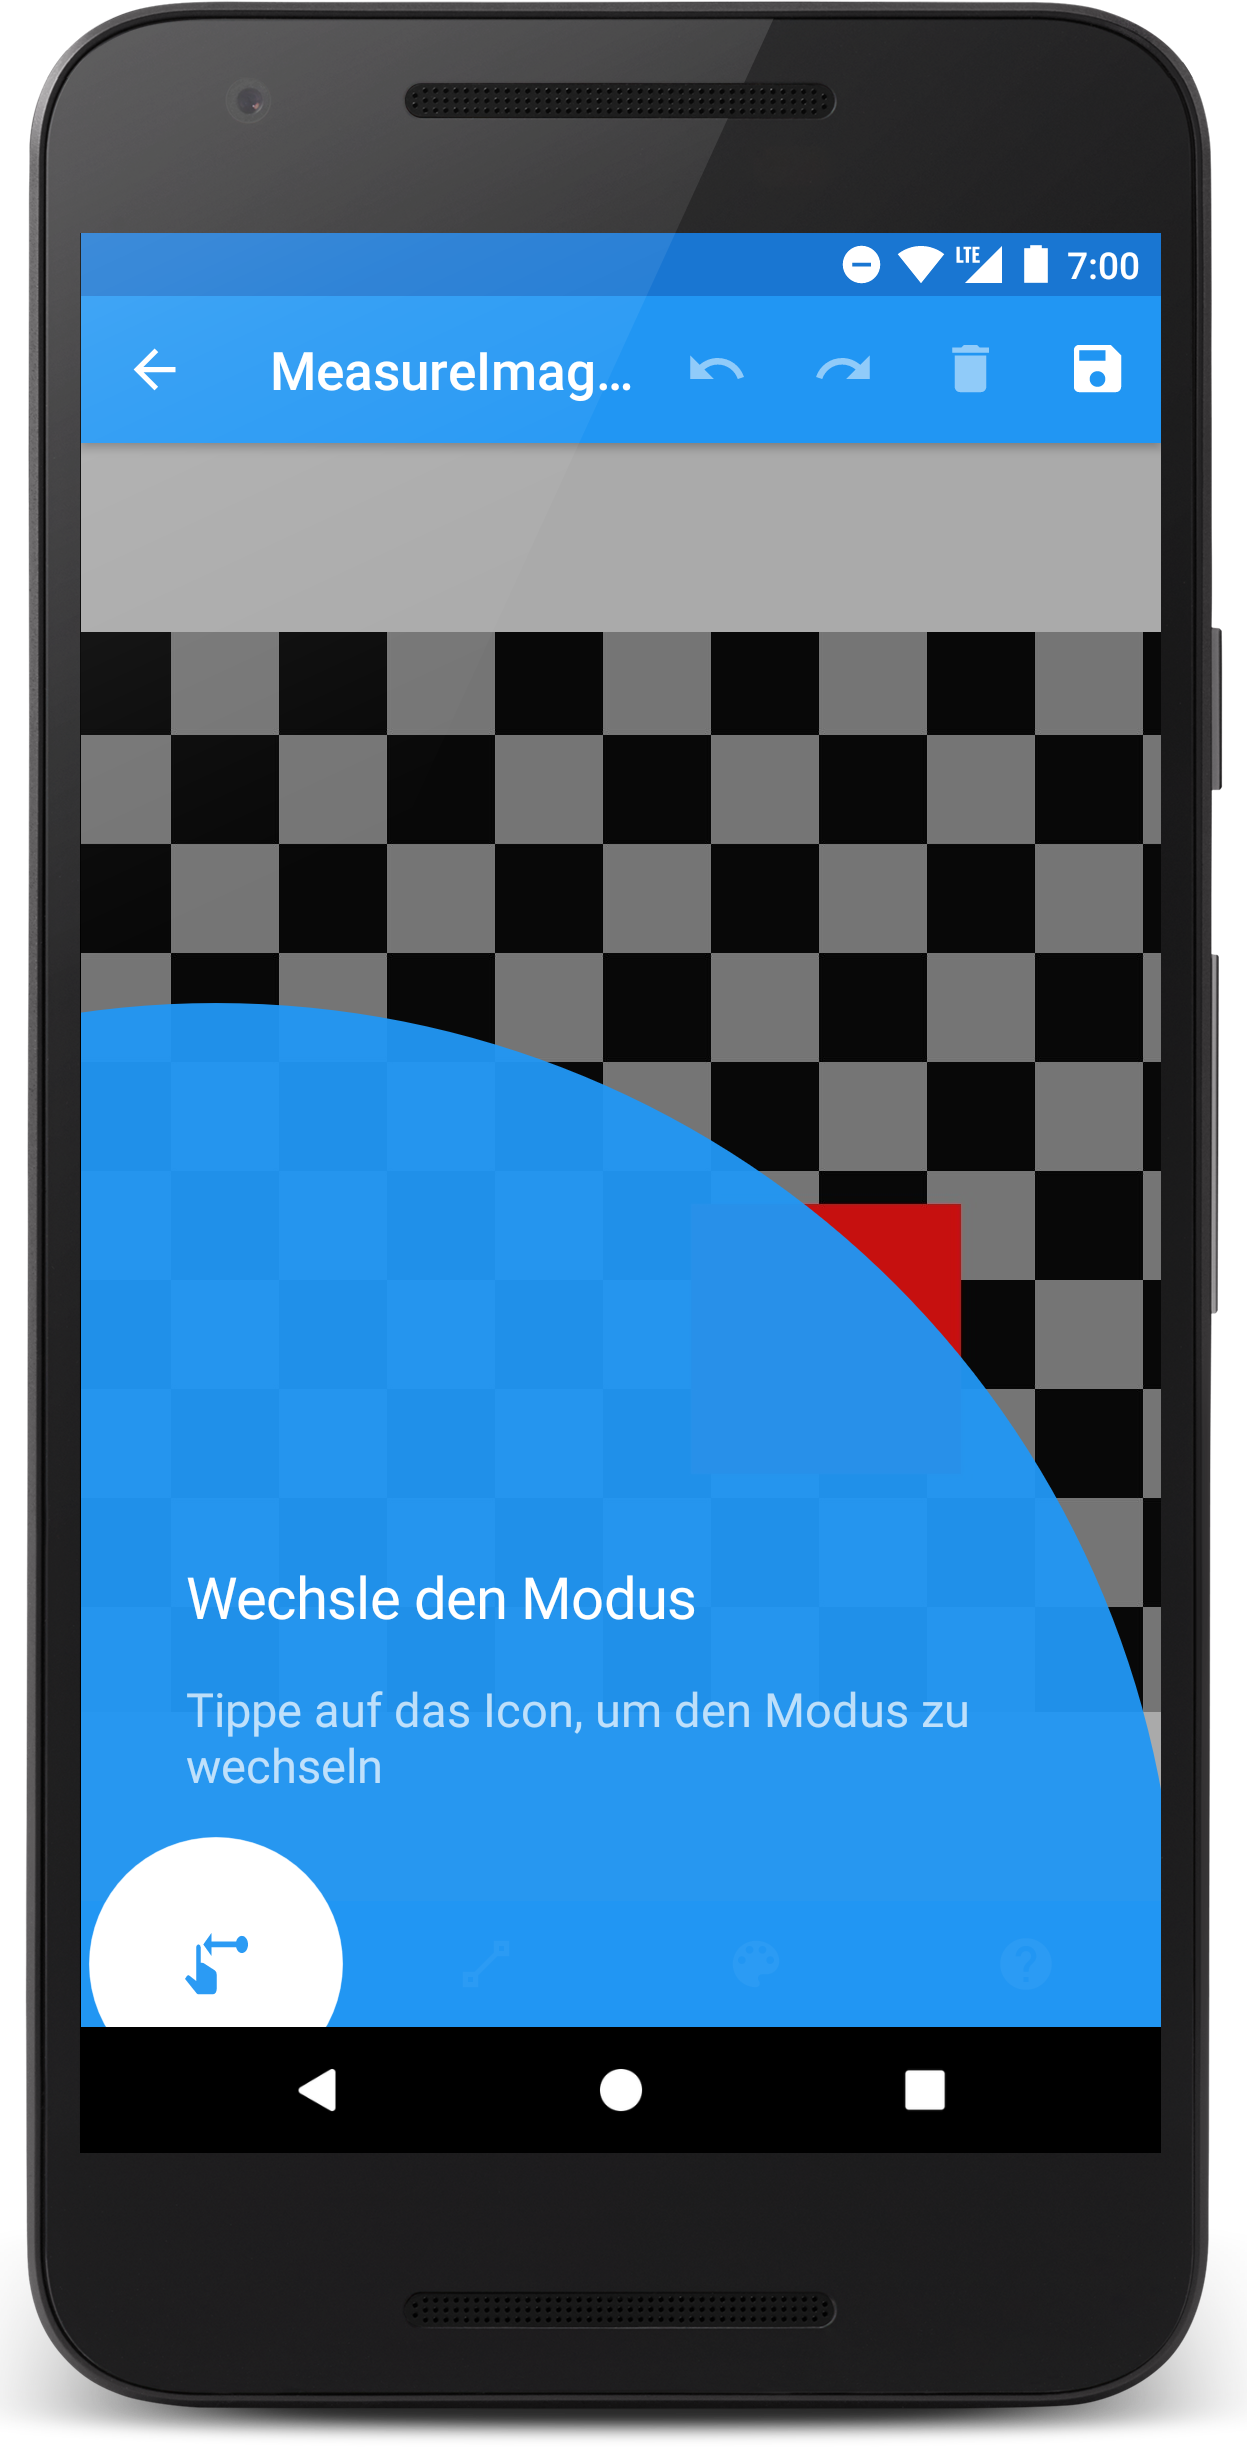
\includegraphics[keepaspectratio, width=\textwidth]{prototype3/help_mode}
    \caption{\emph{Tap-Target} beim initialen Start der App}
    \label{fig:helpmode}
  \end{subfigure}
  \begin{subfigure}[t]{0.3\textwidth}
    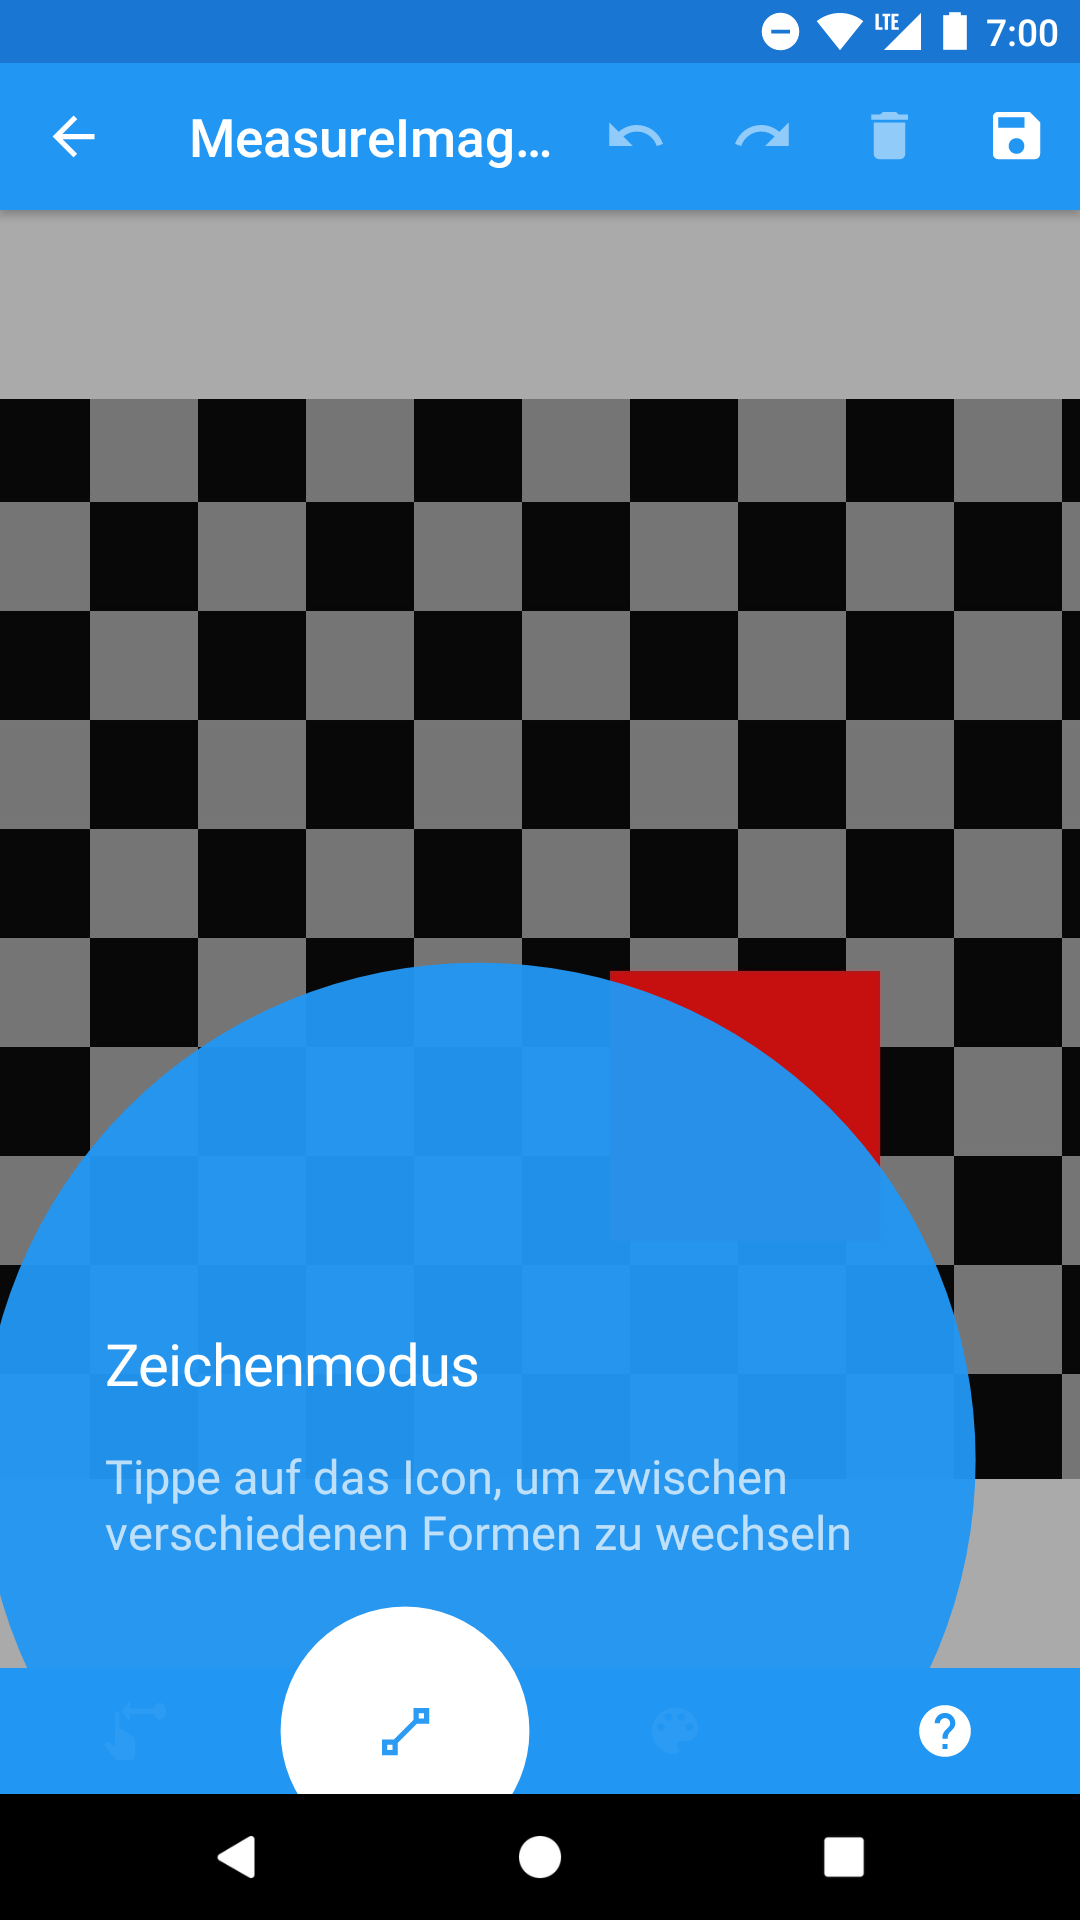
\includegraphics[keepaspectratio, width=\textwidth]{prototype3/help_draw}
    \caption{\emph{Tap-Target} beim initialen Wechsel in den Zeichen-Modus}
    \label{fig:helpdraw}
  \end{subfigure}
  \begin{subfigure}[t]{0.3\textwidth}
    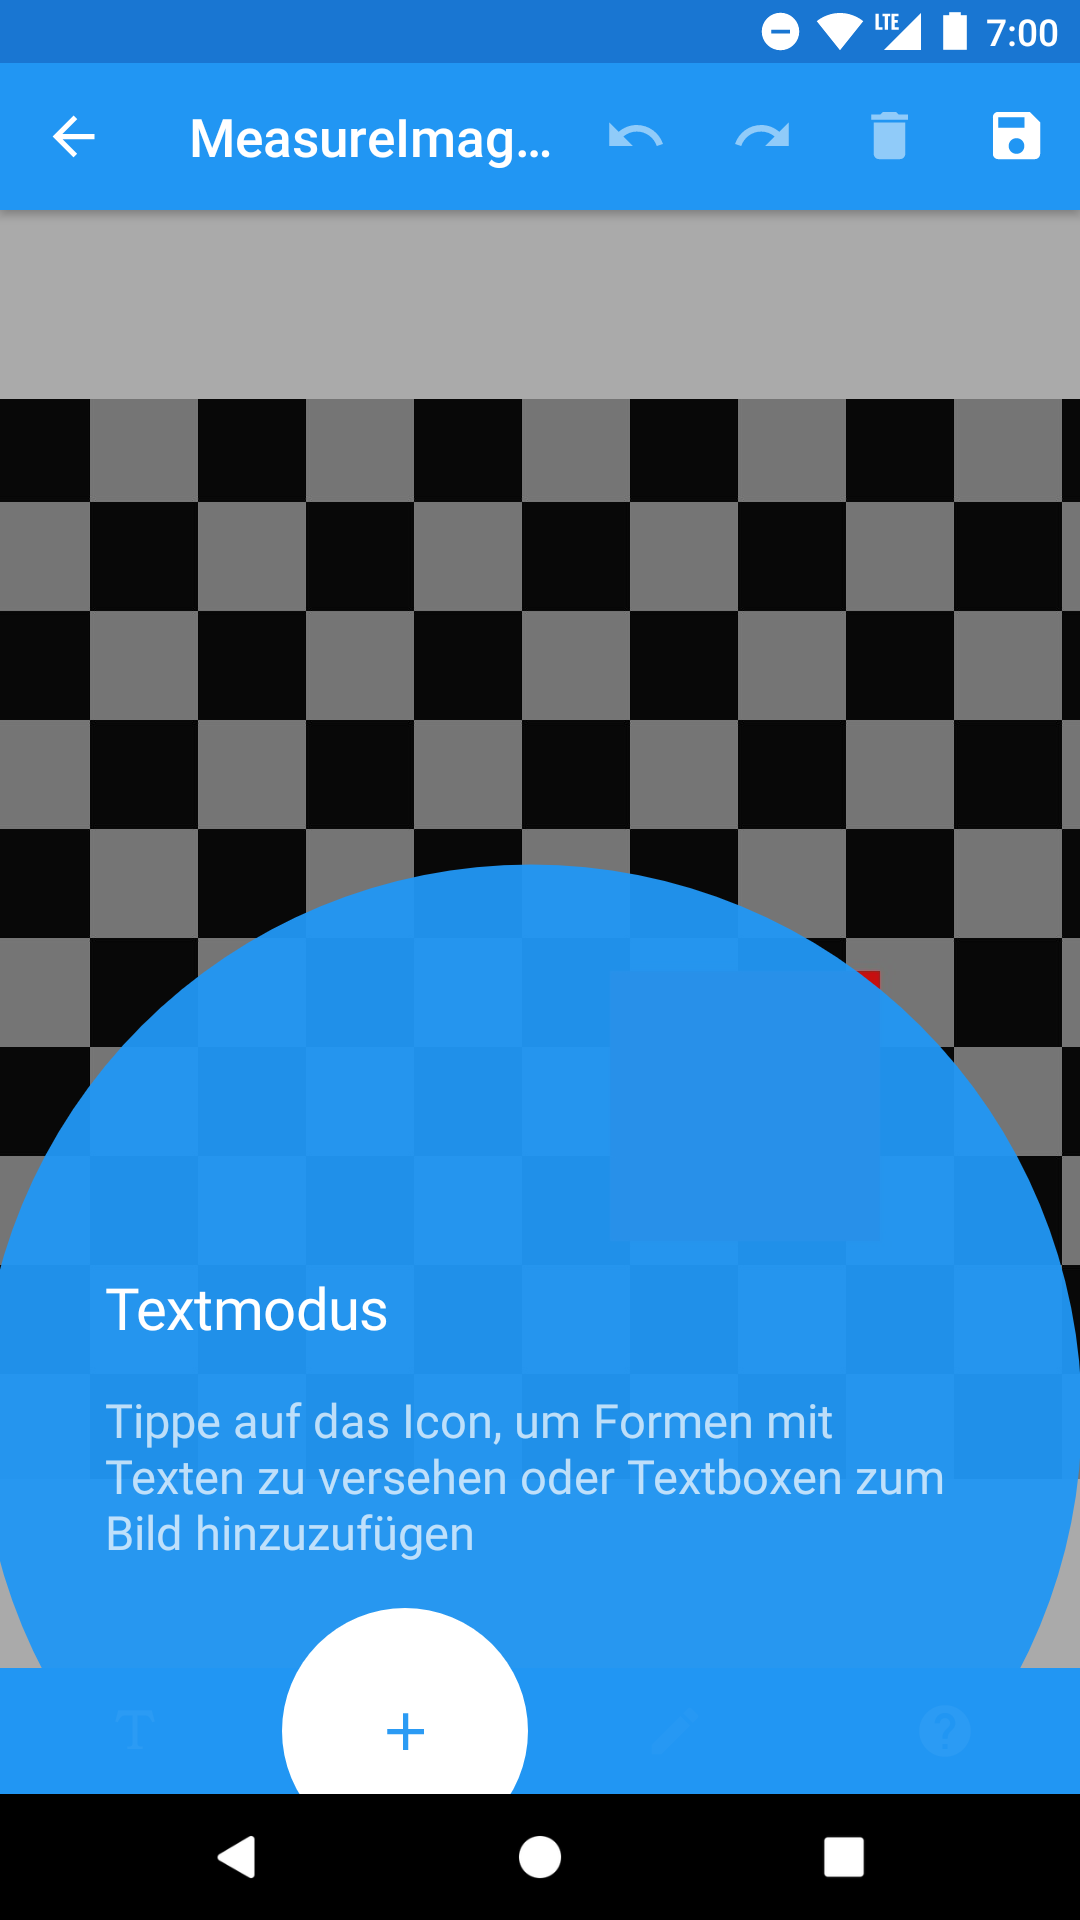
\includegraphics[keepaspectratio, width=\textwidth]{prototype3/help_text}
    \caption{\emph{Tap-Target} beim initialen Wechsel in den Text-Modus}
    \label{fig:helptext}
  \end{subfigure}
  \caption{Die drei verwendeten \emph{Tap-Targets} des dritten Prototyps}
  \label{fig:taptargets}
\end{figure}

Die verwendete \emph{Android-Library} für den Farbdialog\urlnote{https://github.com/jaredrummler/ColorPicker} verfügt bereits über einen ``Preset-Mode'', welcher es ermöglicht, anstatt des gesamten Farbkreises nur eine Farbpalette mit den häufigst genutzten Farben anzuzeigen.
Dieser ``Preset-Mode'' wurde als Standard ausgewählt, und wird beim Öffnen dies Dialogs angezeigt (siehe \autoref{fig:color3}).
Zusätzlich bietet sich dem Benutzer die Möglichkeit über den ``Custom''-Button unten links in die fortgeschrittene Ansicht (siehe \autoref{fig:color1}) zu wechseln. \\

\begin{figure}[h]
  \centering
  \includegraphics[keepaspectratio, width=0.4\textwidth]{prototype3/color}
  \caption{Vereinfachter Farbdialog des dritten Prototyps}
  \label{fig:color3}
\end{figure}

Um mit einem Gerüsttyp verlinkte Formen deutlicher zu kennzeichnen, wurde ein Lineal-Icon hinter die Indikator-Zahl gehangen (siehe \autoref{fig:indicator2}).
Dies soll dazu führen, dass der Nutzer beim Sehen des Indikators direkt den Gerüsttyp-Dialog assoziiert und die Indikator-Zahl nicht mit der Kantenbeschriftung verwechselt.
Zudem wurde in diesem Prototyp die Position des Indikators so verändert, dass dieser neben dem Text der eingetragenen Messwerten steht.
Dies soll verhindern, dass der Indikator einer falschen Form zugeordnet wird, falls Formen auf dem Bild nah nebeneinander liegen. \\

\begin{figure}[h]
  \centering
  \begin{subfigure}[t]{0.4\textwidth}
    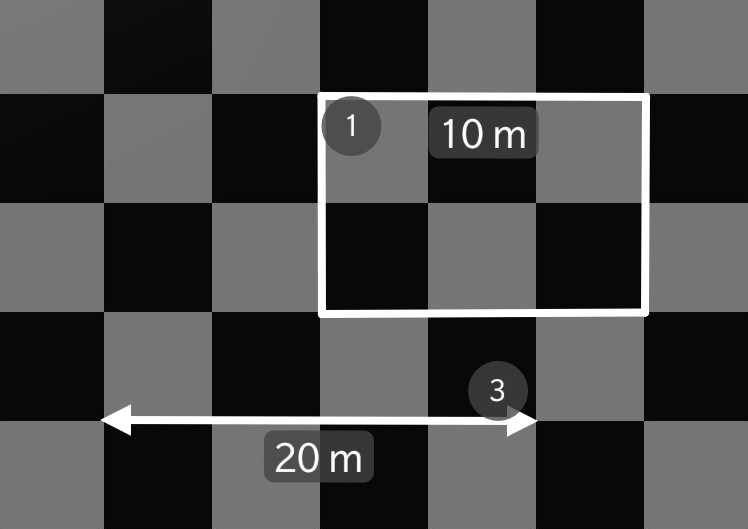
\includegraphics[keepaspectratio, width=\textwidth]{prototype3/indicator1}
    \caption{Gerüsttyp-Indikator im zweiten Prototyp}
    \label{fig:indicator1}
  \end{subfigure}
  \begin{subfigure}[t]{0.4\textwidth}
    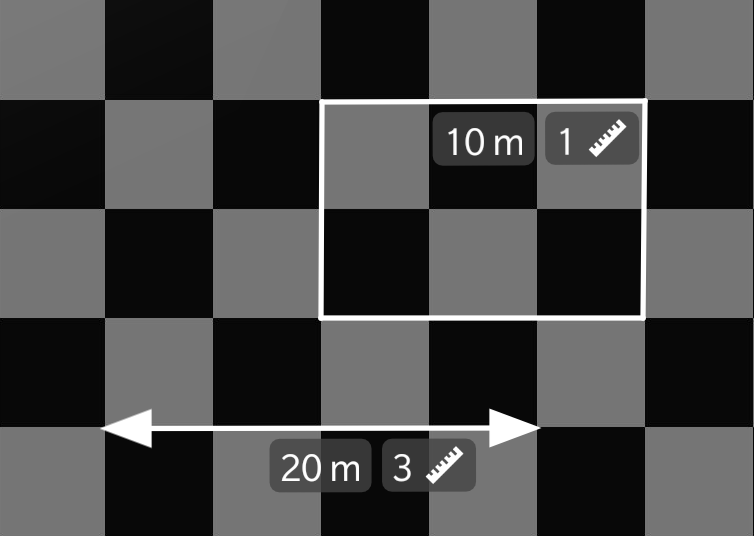
\includegraphics[keepaspectratio, width=\textwidth]{prototype3/indicator2}
    \caption{Gerüsttyp-Indikator im dritten Prototyp}
    \label{fig:indicator2}
  \end{subfigure}
  \caption{Vorher-Nachher-Vergleich des Gerüsttyp-Indikators}
  \label{fig:indicators}
\end{figure}

Im Gerüsttyp-Dialog wurden \emph{AutoCompleteTextField}-Elemente\urlnote{https://developer.android.com/reference/android/widget/AutoCompleteTextView.html} benutzt, welche die eingetragenen Messwerte der Form beim Tippen vorschlagen.
So hat der Nutzer direkt eine Übersicht über die zuvor eingetragenen Messwerte, und muss nicht zwischen Dialog und Bild wechseln. \\

Beide neuen Formen (vgl. \autoref{fig:indicator2}) sind durch Unterklassen, welche von der abstrakten Oberklasse \emph{MeasureShape} erben, modelliert und umgesetzt worden.
Dieser Prozess war für das Hinzufügen der Pfeil-Form trivial, da diese nahezu identisch zu der bereits vorhandenen Linien-Form ist.
Hier wurde lediglich beim Zeichnen der Form eine Pfeilspitze übersprungen.
Bei der Freitext-Form gab es jedoch ein paar Besonderheiten, die zu beachten waren:
Die Freitext-Formen werden im Gegensatz zu allen anderen Formen nicht mit Hilfe einer Zeichen-Geste auf das Bild gezeichnet, sondern sollen in der Mitte der derzeitigen Sichtbereichs erscheinen.
Zudem muss die Größe der Freitext-Form abhängig von der eingegebenen Textlänge dynamisch berechnet und beim Verändern erneut angepasst werden. \\

\section{Testing}\label{sec:test3}
Der dritte Prototyp war 8 Tage in den Arbeitsalltag der beiden Testpersonen integriert, bevor am 24. Januar 2018 Feedback zur Benutzung des Prototyps gesammelt wurde. \\

Die neuen Freitext-Form sei laut Aussage beider Testpersonen in ihrer Funktion nützlich, habe aber den Nachteil, dass wenn mehrere Text-Formen nebeneinander benutzt werden, das Bild schnell unübersichtlich werde. \\

Zudem sei der Dialog zum Speichern des Bildes irritierend, da sowohl im Dialog, als auch in der bestehenden App nach einer Beschreibung für das Bild gefragt wird.
Dies sei ``[\dots] lästig, weil man zweimal den selben Text eintippen muss'' (Testperson 1). \\

Ein weiterer Aspekt, der beiden Testpersonen augefallen ist, sei eine automatische Rotation von aufgenommenen Bildern.
Laut der Tester werden im Hochformat aufgenommene Bilder ins Querformat gedreht, obwohl sie in der Oberfläche zum Schneiden bzw. Rotieren nicht verändert wurden. \\

Diese drei Test-Ergebnisse sollen im nächsten Kapitel in einem vierten Durchlauf des \hcdp{} weiter untersucht und optimiert werden.

\chapter{Vierte Iteration}
Die während der dritten Iteration in \autoref{chap:pro3} identifizierten Usability-Probleme und Anwenderwünsche sollen in diesem Kapitel gelöst werden.
Hierzu wird eine weitere Iteration des \hcdp{} ausgeführt.

\section{Observation}
Um die in \autoref{sec:test3} beschriebenen Probleme hinsichtlich ihrer Entstehung genauer zu evaluieren, werden diese zuerst aufgelistet und anschließend weiter beleuchtet.

\begin{itemize}
  \item Verwendung mehrerer Freitext-Formen im Bild zu unübersichtlich
  \item Doppelte Eingabe des Bildtitles beim Speichern irritierend
\end{itemize}

\noindent
Beide Testpersonen berichten in \autoref{sec:test3} von einer Unübersichtlichkeit bei der Verwendung von mehreren Text-Formen.
Die Schriftgröße des Textes wird dem aktuellen Zoom-Level der App angepasst.
So verkleinert sich der Text, wenn der Nutzer in das Bild hereinzoomt, und vergrößert sich wieder, sobald herausgezoomt wird.
Auf diese Weise soll sichergestellt werden, dass der Text unabhängig vom Zoom-Level jederzeit lesbar ist.
Im herausgezoomten Zustand wird die Schriftgröße jedoch so stark vergrößert, dass die gesamte Text-Form zu viel Platz auf dem Bildschirm einnimmt.
Erstellt der Nutzer jetzt mehrere Text-Formen so kann es schnell passieren, dass diese überlappen, und den gesamten Sichtbereich verdecken.
(Nielsen~\autoref{itm:N12}) \\ 

Außerdem zeigen die Testergebnisse, dass es beim Speichern des bearbeiteten Bildes zu einer doppelten Eingabe des Titels kommt.
So muss der Benutzer einmal beim Speichern des Bildes innerhalb der \emph{Library} eine Beschreibung eingeben, und anschließend ein zweites Mal beim Hochladen des Bildes in der bestehenden App.
Diese doppelte Eingabe der exakt gleichen Beschreibung ist für den Benutzer nicht nachvollziehbar und sorgt drüber hinaus für unnötige Verwirrung.
(Nielsen~\autoref{itm:N1} \& \autoref{itm:N17}) \\ 

\section{Idea Generation}\label{subsec:idea4}
Um das Bild auch bei der Verwendung von mehreren Text-Formen übersichtlich zu halten, bietet es sich an die Textgröße der Formen konfigurierbar zu machen.
Eine Alternative hierzu wäre es, die Formen verkleinerbar zu gestalten, sodass der Nutzer selber entscheiden kann, welche Notiz zu welcher Zeit sichtbar sein soll, und welche zum Beispiel nur als \emph{Icon} auf dem Bild zu sehen ist. \\
\todo{Collapsable Views?}

Die doppelte Eingaben der Bildbeschreibung beim Speichern lässt sich durch das Einführen einer Option in der \emph{Library} lösen, die es der verwendenden App möglich macht, den Speicher-Dialog auszublenden.
So kann bei der bestehenden App der Speicher-Dialog in der \emph{Library} einfach ausgeblendet werden, und so das doppelte Eintragen einer Beschreibung vermieden werden. \\
\todo{Konfigurierabare Libs?}

\section{Prototyping}
Der vierte Prototyp wurde am \todo{Release date nachschauen} ausgerollt und in die bestehende Android-App eingebunden, um die in \autoref{subsec:idea4} genannten Ideen umzusetzen. \\

Für die bessere Übersichtlichkeit bei der Verwendung von mehreren Text-Formen wurde die Funktion implementiert, dass Text-Formen über einen Doppel-Klick ihre Form verändern können.
So werden diese im ``normalen'' Modus wie zuvor als Text-Form mit Hintergrund angezeigt, beim Doppel-Klick transformiert sich diese Form jedoch zu einem kleinen Icon, welches keinerlei Text anzeigt, und nur suggerieren soll, dass sich hier eine Notiz befindet. 
Dies soll dem Benutzer die Möglichkeit geben, selber zu entscheiden, welcher Text wann auf dem Bildschirm sichtbar sein soll und welcher nicht. \\
\todo{Bild mit vielen Texten vorher nachher}

Der Speicher-Dialog wurde durch das Setzen eines optionalen Parameters in der \emph{Library} ausgeblendet, und ist so bei der Benutzung in der bestehenden Android-App nicht mehr zu sehen.
Hier wird das Bild direkt, ohne zuvor nach einer Beschreibung zu fragen, auf dem Handy gespeichert. \\

\section{Testing}
Feedback zur Nutzungserfahrung des vierten Prototyps gab es X Tage nach dem Rollout von den beiden Geschäftsführern. \\

In dieser vierten Iteration des ``Human-Centered Design Process'' seien keine weiteren Probleme bei der Benutzung der App aufgefallen.
Sie ließe sich, so beide Testpersonen, gut und einfach zum Erfassen der Aufmaße verwenden und würde auf langer Sicht viel Arbeit und Zeit sparen, da alle Informationen sofort digital und für jeden verfügbar seien.
\todo{Zitate und abschließend Fazit?}


